
Several applied examples of the IEKF can be found in the literature. Barrau and Bonnabel provide examples of the IEKF applied to two problems in \cite{Barrau2017}. In \cite{Barrau2017aa}, three different applications of the IEKF are presented. However, no results were shown. A case study, clearly demonstrating the geometric advantages of the IEKF is presented in \cite{Barrau2016}. An IEKF applied to scan matching-aided navigation is shown in \cite{Barczyk2016}. A quaternion-based IEKF is applied to a spacecraft attitude estimation problem in \cite{Gui2017}. An IEKF is used as a state estimator for a bipedal robot in \cite{Hartley2018}, which includes bias estimation. The IEKF has also been used to improve on the classic EKF-SLAM solution \cite{Brossard2019}. The popular multi-state constrained Kalman filter \cite{Mourikis2007} is formulated in an invariant framework, including bias estimation, in \cite{Heo2018}. However, some questions remained unanswered. In this chapter, a sample problem is used to illustrate the performance of the IEKF in both simulation and using experimental data. A 3D problem, where the state is an element of $SE(3)$, is considered. The goal of this chapter is to answer four questions left at least partially unanswered in the literature, in order to better explain the practical implications of the IEKF. These questions are as follows.
\begin{enumerate}
	\item Given a left-invariant measurement model, is it more advantageous to use a LIEKF than an MEKF, and given a right-invariant measurement model, is it more advantageous to use a RIEKF than an MEKF?
	
	\item What is the effect of process and measurement noise? How quickly do the convergence properties of the IEKF claimed in \cite{Barrau2017,Barrau2018} break down?
	
	\item How can the IEKF be used in situations when the measurement model isn't left or right-invariant? 
	
	\item How can bias estimation be performed in an invariant framework?
	
\end{enumerate}

To answer the first two questions, a sample problem is presented, followed by some simulation results. The sample problem is then modified in Section \ref{sec:se3_real_data} to fit a realistic measurement model. This new sample problem is then tested on simulated and experimental data. Lastly, the sample problem is once again modified to incorporate bias, followed by simulation results. This will build on the work presented in , \cite{Barrau2015}, \cite{Hartley2018} and \cite{Heo2018}.

\section{\NoAutoSpacing Sample Problem: $SE(3)$}

\subsection{System Modelling}

Consider a body free to translate and rotate in 3D space. Let $\mathcal{F}_a$ be a global frame and $\mathcal{F}_b$ be a frame which rotates with the body. Point $z$ moves with the body, while point $w$ is a reference point. The problem setup is illustrated in Figure~\ref{fig:se3_prob}.
\begin{figure}
	\centering
	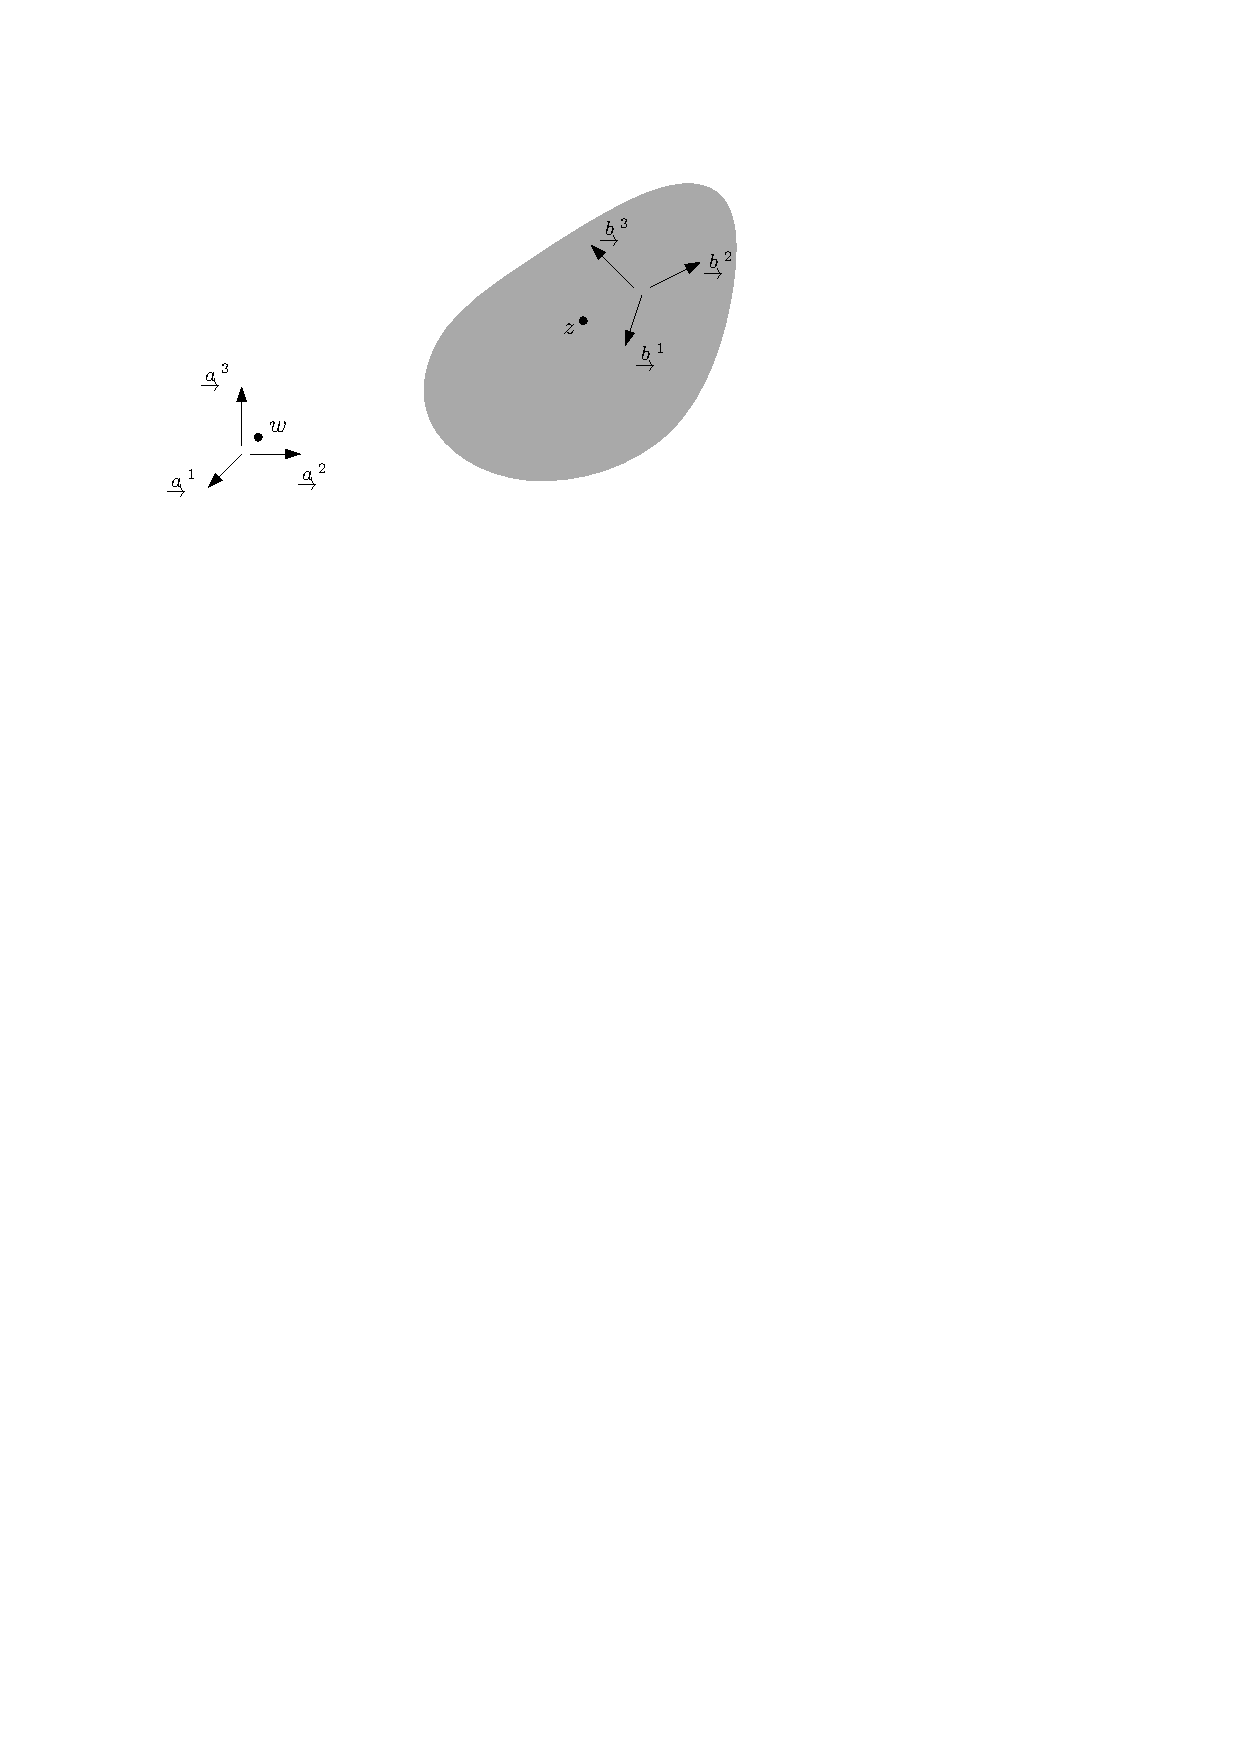
\includegraphics[width=0.7\textwidth]{figs/prob.pdf}
	\caption[Problem setup.]{Problem setup.}
	\label{fig:se3_prob}
\end{figure}
The estimated states are $\mbf{r}_a^{zw}$ and $\mbf{C}_{ab}$. The pose can be represented as an element of $SE(3)$ as
\bdis
	\mbf{T}_{ab} = 
	\bma{cc}
		\mbf{C}_{ab} & \mbf{r}_a^{zw} \\
		\mbf{0} & 1
	\ema.
\edis The kinematics of this problem are
\begin{align*}
	\mbfdot{C}_{ab} &= \mbf{C}_{ab} \mbs{\omega}_b^{{ba}^\times}, \\
	\mbfdot{r}_a^{zw} &= \mbf{v}_a^{zw/a}.
\end{align*}
In matrix form, the kinematics are 
\bdis
	\mbfdot{T}_{ab} = \mbf{T}_{ab}\mbs{\varpi}_b^\wedge,
\edis
where $\mbs{\varpi}_b = \left[ \; {\mbs{\omega}_b^{ba}}^\trans \; {\mbf{v}_b^{zw/a}}^\trans \; \right]^\trans$. 
The body is equipped with a rate gyro which measures
\bdis
	\mbf{u}_b^1 = \mbs{\omega}_b^{ba} - \mbf{w}_b^1,
\edis
where $\mbf{w}_{b}^1$ is band-limited white noise. When discretized, $\mbf{w}_{b_k}^1 \sim \mathcal{N}\left(0,\mbf{Q}_k^1\right)$.  The body is also equipped with a velocity sensor that measures
\bdis
	\mbf{u}_b^2 = \mbf{v}_{b}^{zw/a} - \mbf{w}_b^2,
\edis
where $\mbf{w}_{b}^2$ is band-limited white noise. When discretized, $\mbf{w}_{b_k}^2 \sim \mathcal{N}\left(0,\mbf{Q}_k^2\right)$. Rearranging and substituting into the kinematics leads to
\begin{align*}
	\mbfdot{C}_{ab} &= \mbf{C}_{ab} \left(\mbf{u}_b^1 + \mbf{w}_b^1\right)^\times, \\
	\mbfdot{r}_a^{zw} &= \mbf{C}_{ab} \left(\mbf{u}_b^2 +  \mbf{w}_b^2 \right).
\end{align*}
Incorporating the measurement model, the kinematics in matrix form are 
\bdis
	\mbfdot{T}_{ab} = \mbf{T}_{ab}\left(\mbf{u}_b +  \mbf{w}_b \right)^\wedge,
\edis
where $\mbf{u}_b = \left[ \; {\mbf{u}_b^1}^\trans \; {\mbf{u}_b^2}^\trans \; \right]^\trans$ and $\mbf{w}_b = \left[ \; {\mbf{w}_b^1}^\trans \; {\mbf{w}_b^2}^\trans \; \right]^\trans$. Throughout this chapter, the subscripts on $\mbf{T}_{ab}$ are dropped to be concise.


\subsection{Left-Invariant Extended Kalman Filter Derivation}
\label{ssec:se3_LIEKF}

In order to derive a LIEKF, the exteroceptive measurement model must be left invariant. In this case, approriate measurements are position measurements, which could be from a GPS receiver, for example. The discrete-time measurement model is
\beq
	\bma{c} \mbf{y}_{a_k} \\ 0 \ema = \bma{c} \mbf{r}_a^{z_k w} +  \mbf{v}_{a_k} \\ 1 \ema = \mbf{T}_k
	\bma{c}
		\mbf{0} \\
		1
	\ema
	+ 
	\bma{c}
		\mbf{v}_{a_k} \\
		0
	\ema, \label{eq:se3_meas_left}
\eeq
where $\mbf{v}_{a_k} \sim \mathcal{N}\left(\mbf{0},\mbf{R}_k\right)$. 

The left-invariant error  $\mbfdel{T} = \mbf{T}^{-1}\mbfhat{T}$ is used because the measurement model is left invariant. The error propagation is 
\begin{align} 
	\delta \mbfdot{T} & = \mbfdot{T}^{-1} \mbfhat{T} + \mbf{T}^{-1}\dot{\mbfhat{T}} \nonumber \\
	& = -\mbf{T}^{-1} \mbfdot{T} \mbf{T}^{-1} \mbfhat{T} + \mbf{T}^{-1} \mbfhat{T} \mbf{u}_b^\wedge \nonumber \\
	& = -\mbf{T}^{-1} \mbf{T} \left(\mbf{u}_b + \mbf{w}_b\right)^\wedge \mbf{T}^{-1} \mbfhat{T} + \mbfdel{T} \mbf{u}_b^\wedge \nonumber \\
	& = -\left(\mbf{u}_b + \mbf{w}_b\right)^\wedge  \mbfdel{T} + \mbfdel{T} \mbf{u}_b^\wedge  \label{eq:se3_left_1}.
\end{align}
To linearize \eqref{eq:se3_left_1}, let $\mbfdel{T} \approx \mbf{1} + \mbsdel{\xi}^\wedge$, $\mbfdel{T}^{-1} \approx \mbf{1} - \mbsdel{\xi}^\wedge$,  and $\mbf{w}_b = \mbfdel{w}_b$. Neglecting second order terms, \eqref{eq:se3_left_1} is then approximated as
\begin{align} 
	\f{\dee}{\dt} \left(\mbf{1} + \mbsdel{\xi}^\wedge\right) & = \left(\mbf{1} + \mbsdel{\xi}^\wedge\right) \mbf{u}_b^\wedge -\left(\mbf{u}_b + \mbfdel{w}_b\right)^\wedge \left(\mbf{1} +\mbsdel{\xi}^\wedge\right), \nonumber \\
	\delta \mbsdot{\xi}^\wedge & = \mbf{u}_b^\wedge + \mbsdel{\xi}^\wedge \mbf{u}_b^\wedge - \left(\mbf{u}_b + \mbfdel{w}_b\right)^\wedge - \left(\mbf{u}_b + \mbfdel{w}_b\right)^\wedge \mbsdel{\xi}^\wedge \nonumber \\
	 & = \mbsdel{\xi}^\wedge \mbf{u}_b^\wedge - \mbf{u}_b^\wedge \mbsdel{\xi}^\wedge -\mbfdel{w}_b^\wedge .  \label{eq:se3_left_2}
\end{align}
Using the identity \eqref{eq:ad_identity}, \eqref{eq:se3_left_2} is rewritten as
\bdis
	\delta \mbsdot{\xi}^\wedge = \left(-\textrm{ad}(\mbf{u}_b) \mbsdel{\xi}\right)^\wedge - \mbfdel{w}_b^\wedge,
\edis
which in turn can be written as
\bdis
	\delta \mbsdot{\xi} = -\textrm{ad}(\mbf{u}_b) \mbsdel{\xi} - \mbfdel{w}_b.
\edis
Therefore, $\mbf{A} = -\textrm{ad}(\mbf{u}_b)$ and $\mbf{L} = -\mbf{1}$. Notice that $\mbf{A}$ is only a function of the measurement $\mbf{u}_b$.

When a position measurement $\mbf{y}_{a_k}$ is available, the state estimate is corrected. This correction has the form
\bdis
	\mbfhat{T}_k = \mbfcheck{T}_k\exp\left(-\left(\mbf{K}_k\mbf{z}_k\right)^\wedge\right) .
\edis
The innovation is
\begin{align}
	\bma{c} \mbf{z}_k \\ 0 \ema &= \mbfcheck{T}_k^{-1}\left(\bma{c} \mbf{y}_{a_k} \\ 1 \ema - \bma{c} \mbfcheck{y}_{a_k} \\ 1 \ema\right) \nonumber \\
	&= \mbfcheck{T}_k^{-1} \left(\mbf{T}_k \bma{c} \mbf{0} \\	1 \ema + \bma{c} \mbf{v}_{a_k} \\0 \ema - \mbfch{T}_k \bma{c} \mbf{0} \\ 1 	\ema \right) \nonumber \\
	&= \delta \mbfch{T}_k^{-1} \bma{c} \mbf{0} \\	1 \ema + \mbfch{T}_k^{-1}\bma{c} \mbf{v}_{a_k} \\0 \ema - \bma{c} \mbf{0} \\ 1 \ema. \label{eq:se3_left_3}
\end{align}
Linearizing \eqref{eq:se3_left_3} by letting  $\delta \mbfcheck{T}_k^{-1} \approx \mbf{1} - \delta \mbscheck{\xi}_k^\wedge$ and $\mbf{v}_{a_k} = \mbfdel{v}_{a_k}$,
\begin{align}
	\bma{c} \mbf{z}_k \\ 0 \ema &\approx \left(\mbf{1} - \delta \mbscheck{\xi}_k^\wedge\right) 
\bma{c}
	\mbf{0} \\
	1
\ema +
\mbfcheck{T}_k^{-1}
\bma{c}
	\mbfdel{v}_{a_k} \\
	0
\ema - 	
\bma{c}
	\mbf{0} \\
	1
\ema \nonumber \\
	& = -\delta \mbscheck{\xi}_k^\wedge 
\bma{c}
	\mbf{0} \\
	1
\ema + \mbfcheck{T}_k^{-1}
\bma{c}
	\mbfdel{v}_{a_k} \\
	0
\ema \nonumber \\
	& =  
-\bma{cc}
	{\delta\mbscheck{\xi}^\phi}^\times & \delta\mbscheck{\xi}_k^\textrm{r} \\
 	\mbf{0} & 0 
\ema 
\bma{c}
	\mbf{0} \\
	1
\ema + \mbfcheck{T}_k^{-1}
\bma{c}
	\mbfdel{v}_{a_k} \\
	0
\ema \nonumber \\
	& =  
	\mbftilde{H} \delta \mbscheck{\xi}_k + \mbfcheck{T}_k^{-1}
\bma{c}
	\mbfdel{v}_{a_k} \\
	0
\ema , \label{eq:se3_left_4}
\end{align}
where 
\bdis
	\mbftilde{H} = 
	\bma{cc}
		\mbf{0} & -\mbf{1} \\
		\mbf{0} & \mbf{0}
	\ema.
\edis
Noting that the bottom row of \eqref{eq:se3_left_4} is only zeros, it can be written
\bdis
	\mbf{z}_k = \mbf{H} \delta \mbscheck{\xi}_k + \mbf{M}_k \mbfdel{v}_{a_k}
\edis
where
\bdis
	\mbf{H} = 
	\bma{cc}
		\mbf{0} & -\mbf{1} \\
	\ema
\edis
and $\mbf{M}_k = \mbfch{C}_{ab_k}^\trans$. Notice that $\mbf{H}$ is constant.

\subsection{Right-Invariant Extended Kalman Filter Derivation}
\label{ssec:SE3_RIEKF}

In order to derive a RIEKF, the exteroceptive measurement model must be right invariant. In this case, appropriate measurements are landmark measurements resolved in (i.e. observed in) the body frame, which could be from a LIDAR or camera, for example. In reality, the measurement model depends on the sensor. However, for the sake of simplicity, the exteroceptive measurements are modelled as relative landmark locations. This ensures the measurement model is actually right-invariant. Let point $p^i$ be associated with the $i^{th}$ landmark. The position of the $i^{th}$ landmark relative to point $w$ resolved in $\rframe{a}$ is $\mbf{r}_a^{p_iw}$. The landmark sensor is assumed to measure $\mbf{r}_b^{p_iz}$. Figure~\ref{fig:se3_prob_landmarks} displays the geometry of the problem. 
\begin{figure}
	\centering
	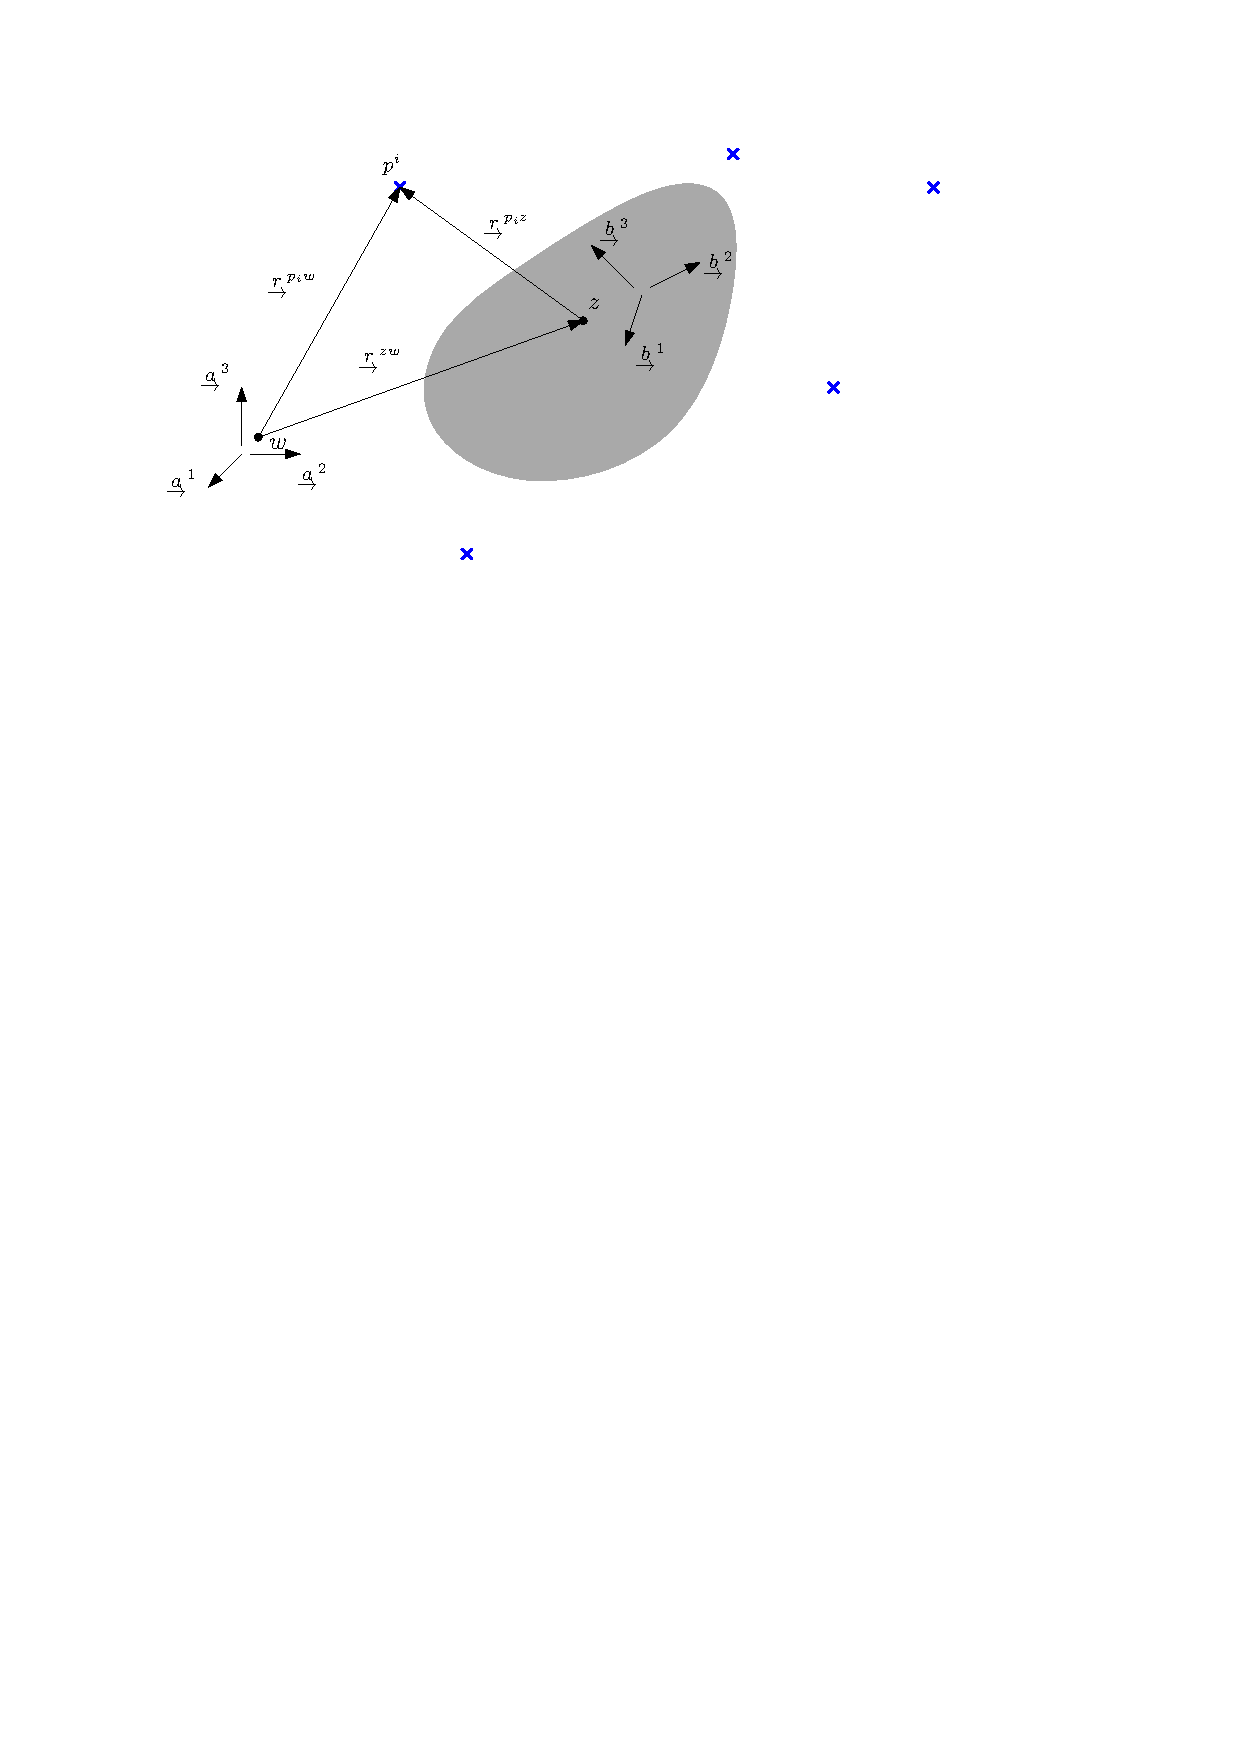
\includegraphics[width=0.7\textwidth]{figs/prob_landmarks.pdf}
	\caption{Problem setup, where the blue crosses are the observed landmarks.}
	\label{fig:se3_prob_landmarks}
\end{figure}
The discrete-time measurement model is then
\beq
	\bma{c} \mbf{y}_{b_k}^i \\ 1 \ema = \bma{c} \mbf{C}_{ab_k}^\trans\left( \mbf{r}_a^{p_iw} - \mbf{r}_a^{z_k w} \right) +  \mbf{v}_{b_k}^i \\ 1 \ema = \mbf{T}_k^{-1}
	\bma{c}
		 \mbf{r}_a^{p_iw}\\
		1
	\ema
	+ 
	\bma{c}
		\mbf{v}_{b_k}^i \\
		0
	\ema, \label{eq:se3_meas_right}
\eeq
where $\mbf{v}_{b_k}^i \sim \mathcal{N}\left(\mbf{0},\mbf{R}_k^i\right)$, $i = 1,\ldots,m$, where $m$ is the number of landmarks.

The right-invariant error  $\mbfdel{T} = \mbfhat{T}\mbf{T}^{-1}$ is used. The error propagation is
\begin{align} 
	\delta \mbfdot{T} & = \dot{\mbfhat{T}}\mbf{T}^{-1}  + \mbfhat{T}\mbfdot{T}^{-1} \nonumber \\
	& = \mbfhat{T} \mbf{u}_b^\wedge\mbf{T}^{-1}   - \mbfhat{T}\mbf{T}^{-1} \mbfdot{T} \mbf{T}^{-1} \nonumber \\
	& = \mbfhat{T} \mbf{u}_b^\wedge\mbf{T}^{-1}  - \mbfhat{T}\mbf{T}^{-1}\mbf{T}\left(\mbf{u}_b + \mbf{w}_b\right)^\wedge \mbf{T}^{-1}  \nonumber \\
	& = \mbfhat{T} \left(\mbf{u}_b - \mbf{u}_b - \mbf{w}_b\right)^\wedge \mbf{T}^{-1}  \nonumber \\
	& = -\mbfhat{T}\mbf{w}_b^\wedge\mbfhat{T}^{-1}\mbfdel{T}  \nonumber \\
	& = -\left(\textrm{Ad}(\mbfhat{T})\mbf{w}_b\right)^\wedge\mbfdel{T}  \label{eq:se3_right_1}.
\end{align}
To linearize \eqref{eq:se3_right_1}, let $\mbfdel{T} \approx \mbf{1} + \mbsdel{\xi}^\wedge$  and $\mbf{w}_b = \mbfdel{w}_b$. Neglecting second order terms, \eqref{eq:se3_right_1} is then 
\begin{align} 
	\f{\dee}{\dt} \left(\mbf{1} + \mbsdel{\xi}^\wedge\right) & = -\left(\textrm{Ad}(\mbfhat{T})\mbfdel{w}_b\right)^\wedge\left(\mbf{1} +\mbsdel{\xi}^\wedge\right), \nonumber \\
	\delta \mbsdot{\xi}^\wedge & = -\left(\textrm{Ad}(\mbfhat{T})\mbfdel{w}_b\right)^\wedge, \nonumber \\
	\delta \mbsdot{\xi} & = -\textrm{Ad}(\mbfhat{T})\mbfdel{w}_b.  \label{eq:se3_right_2}
\end{align}
Therefore, $\mbf{A} = \mbf{0}$ and $\mbf{L} =  -\textrm{Ad}(\mbfhat{T})$. Notice that $\mbf{A}$ is constant.		

\mymargin{Edited 2021/2/17} 
When a relative landmark measurement $\mbf{y}_{b_k}^i$ is available, the state estimate is corrected. This correction has the form
\bdis
	\mbfhat{T}_k =  \exp\left(-\left(\mbf{K}_k\mbf{z}_k\right)^\wedge\right)\mbfcheck{T}_k.
\edis
The innovation associated with the $i^{th}$ landmark is
\begin{align}
	\bma{c} \mbf{z}_k^i \\ 0 \ema &= \mbfcheck{T}_k\left(\bma{c} \mbf{y}_{b_k}^i \\ 1 \ema - \bma{c} \mbfcheck{y}_{b_k}^i \\ 1 \ema\right) \nonumber \\
	&= \mbfcheck{T}_k \left(\mbf{T}_k^{-1} \bma{c} \mbf{r}_a^{p_iw} \\	1 \ema + \bma{c} \mbf{v}_{b_k}^i \\0 \ema - \mbfch{T}_k^{-1} \bma{c} \mbf{r}_a^{p_iw} \\ 1 	\ema \right) \nonumber \\
	&= \delta \mbfch{T}_k \bma{c} \mbf{r}_a^{p_iw} \\	1 \ema + \mbfch{T}_k\bma{c} \mbf{v}_{b_k}^i \\0 \ema - \bma{c} \mbf{r}_a^{p_iw} \\ 1 \ema. \label{eq:se3_right_3}
\end{align}
Linearizing \eqref{eq:se3_right_3} by letting  $\delta \mbfcheck{T}_k \approx \mbf{1} + \delta \mbscheck{\xi}_k^\wedge$ and $\mbf{v}_{b_k} = \mbfdel{v}_{b_k}$,
\begin{align}
	\bma{c} \mbf{z}_k^i \\ 0 \ema &\approx \left(\mbf{1} + \delta \mbscheck{\xi}_k^\wedge\right) 
\bma{c}
	\mbf{r}_a^{p_iw} \\
	1
\ema +
\mbfcheck{T}_k
\bma{c}
	\mbfdel{v}_{b_k}^i \\
	0
\ema - 	
\bma{c}
	\mbf{r}_a^{p_iw} \\
	1
\ema \nonumber \\
	& = \delta \mbscheck{\xi}_k^\wedge 
\bma{c}
	\mbf{r}_a^{p_iw} \\
	1
\ema + \mbfcheck{T}_k
\bma{c}
	\mbfdel{v}_{b_k}^i \\
	0
\ema \nonumber \\
	& =  
\bma{cc}
	{\delta\mbscheck{\xi}_k^{\phi}}^\times & \delta\mbscheck{\xi}_k^\textrm{r} \\
 	\mbf{0} & 0 
\ema 
\bma{c}
	\mbf{r}_a^{p_iw} \\
	1
\ema + \mbfcheck{T}_k
\bma{c}
	\mbfdel{v}_{b_k}^i \\
	0
\ema \nonumber \\
	& =  
\bma{c}
	{\delta\mbscheck{\xi}_k^{\phi}}^\times\mbf{r}_a^{p_iw} + \delta\mbscheck{\xi}_k^\textrm{r} \\
 	\mbf{0} 
\ema 
 + \mbfcheck{T}_k
\bma{c}
	\mbfdel{v}_{b_k}^i \\
	0
\ema \nonumber \\
	& =  
\bma{c}
	-{\mbf{r}_a^{p_iw}}^\times{\delta\mbscheck{\xi}_k^{\phi}} + \delta\mbscheck{\xi}_k^\textrm{r} \\
 	\mbf{0} 
\ema 
 + \mbfcheck{T}_k
\bma{c}
	\mbfdel{v}_{b_k}^i \\
	0
\ema \nonumber \\
	& =  
	\mbf{H}^i \delta \mbscheck{\xi}_k + \mbfcheck{T}_k
\bma{c}
	\mbfdel{v}_{b_k}^i \\
	0
\ema , \label{eq:se3_right_4}
\end{align}
where 
\bdis
	\mbftilde{H} = 
	\bma{cc}
		-{\mbf{r}_a^{p_iw}}^\times & \mbf{1} \\
		\mbf{0} & \mbf{0}
	\ema.
\edis
Noting that the bottom row of \eqref{eq:se3_right_4} is full of zeros, it can be written
\bdis
	\mbf{z}_k^i = \mbf{H}^i \delta \mbscheck{\xi}_k + \mbf{M}_k \mbfdel{v}_{b_k}^i
\edis
where
\bdis
	\mbf{H}^i = 
	\bma{cc}
		-{\mbf{r}_a^{p_iw}}^\times & \mbf{1} \\
	\ema
\edis
and $\mbf{M}_k = \mbfch{C}_{ab_k}^\trans$. For the $m$ landmarks,
\beq
	\mbf{H} = \underset{i = 1,\ldots,m}{\textrm{row}}\left(
	\bma{cc}
		-{\mbf{r}_a^{p_iw}}^\times & \mbf{1} \\
	\ema
	\right) \label{eq:se3_H_riekf}
\eeq
and $\mbf{M}_k = \textrm{diag}\left(\mbfcheck{C}_{ab_k}^\trans,\ldots,\mbfcheck{C}_{ab_k}^\trans\right)$. Once again, notice that $\mbf{H}$ is constant, because $\mbf{r}_a^{p_i w} ,  i = 1,  \ldots , m$ are constant and known a priori.

\subsection{MEKF Solutions}
\label{ssec:se3_EKF}

Throughout this section, the results are compared to that of a standard multiplicative extended Kalman filter (MEKF). A MEKF is a variant of the EKF better suited for attitude estimation. The Jacobians for the MEKF are presented here, but no derivation is given. The errors are defined as $\mbfdel{C} = \mbfbar{C}_{ab}^\trans\mbf{C}_{ab}$ and $\mbfdel{r} = \mbf{r}_a^{zw} - \mbfbar{r}_a^{zw}$. Two different MEKFs must be used for the two different measurement models. The first MEKF, which uses the left-invariant measurements \eqref{eq:se3_meas_left}, is referred to as MEKF-L. The MEKF using the right-invariant measurements \eqref{eq:se3_meas_right} is referred to as MEKF-R. The process model Jacobians for both are
\bdis
	\mbf{A} = 
	\bma{cc}
		-{\mbf{u}_b^1}^\times & \mbf{0} \\
		-\mbfhat{C}_{ab}{\mbf{u}_b^2}^\times & \mbf{0}
	\ema,
	\quad
	\mbf{L} = 
	\bma{cc}
		\mbf{1} & \mbf{0} \\
		\mbf{0} & \mbfhat{C}_{ab}
	\ema.
\edis
Note that $\mbf{A}$ depends on the attitude estimate, which was not the case for the IEKFs. For the MEKF-L, the measurement model Jacobians are
\bdis
	\mbf{H} = 
	\bma{cc}
		\mbf{0} & \mbf{1} \\
	\ema,
	\quad
	\mbf{M} = \mbf{1}.
\edis
For the MEKF-R, the measurement model Jacobians are
\bdis
	\mbf{H}_k^i = 
	\bma{cc}
		 \left(\mbfch{C}_{ab_k}^\trans\left( \mbf{r}_a^{p_iw} - \mbfch{r}_a^{z_k^i w} \right)\right)^\times & -\mbfch{C}_{ab_k}^\trans \\
	\ema,
	\quad
	\mbf{M} = \mbf{1}.
\edis
For the $m$ landmarks,
\beq
	\mbf{H}_k = \underset{i = 1,\ldots,m}{\textrm{row}}\left(
	\bma{cc}
		  \left(\mbfch{C}_{ab_k}^\trans\left( \mbf{r}_a^{p_iw} - \mbfch{r}_a^{z_k^i w} \right)\right)^\times & -\mbfch{C}_{ab_k}^\trans \\
	\ema
	\right) \label{eq:se3_H_ekf}
\eeq
and $\mbf{M} = \mbf{1}$. The MEKF-R's measurement model Jacobian $\mbf{H}_k$ depends on the state estimate, which was not the case for the RIEKF.

\subsection{Simulation Results}

In this section, simulations are performed to compare the four Kalman filters shown in Sections~\ref{ssec:se3_LIEKF}, \ref{ssec:SE3_RIEKF}, and \ref{ssec:se3_EKF}, namely the LIEKF, RIEKF, MEKF-L and MEKF-R. The first question raised in the introduction of this chapter asked whether it was advantageous to use an invariant filter over its standard multiplicative counterpart. The second question concerns the effect of noise on the theoretical convergence properties of the IEKF. The two questions are simultaneously addressed in this section. 

\subsubsection{Simulation Parameters}

In one set of trials, the MEKF-L and LIEKF are compared. In another, the RIEKF and MEKF-R are compared. Certain parameters are kept constant throughout the simulation. The trajectory used is shown in Figure~\ref{fig:se3_traj}. The landmarks used in the RIEKF and MEKF-R are also displayed. It is assumed that, at any given time, all the landmarks are visible. The rate gyro and velocity sensor operate at \SI{100}{\Hz}, while the corrections occur at \SI{10}{\Hz}. The trajectory is parametrized such that $\norm{\mbf{v}_b^{zw/a}}$ is constant at \SI{1}{m/s}. The resulting trajectory takes slightly over \SI{30}{\second} to execute, which is generally enough time for the transients associated with the convergence of the filters to dissipate. The attitude is constrained to have constant roll. To simplify the situation, the sensor noise is assumed isotropic. That is, $\mbf{Q}_k^1 = {\sigma_k^1}^2\mbf{1}$, $\mbf{Q}_k^2 = {\sigma_k^2}^2\mbf{1}$, and $\mbf{R}_k^i = {\sigma_k^\textrm{R}}^2\mbf{1}$. Doing this makes the fact $\mbf{M}_k$ may depend on $\mbfch{C}_{ab_k}$ irrelevant because $\mbf{M}_k^\trans\mbf{R}_k \mbf{M}_k = \mbf{R}_k$ thereby making the computation of the Kalman gain independent of $\mbf{M}_k$. In many applications, the covariance matrices are seen as tuning parameters. Here, no tuning is done. Tuning may greatly effect the results, but in simulation, keeping the theoretical values is more valuable because it demonstrates how the filters behave ``out of the box'' without extensive tuning. 
%  Trajectory
\begin{figure}
 \centering
        \begin{subfigure}[b]{0.495\textwidth}
            \centering
            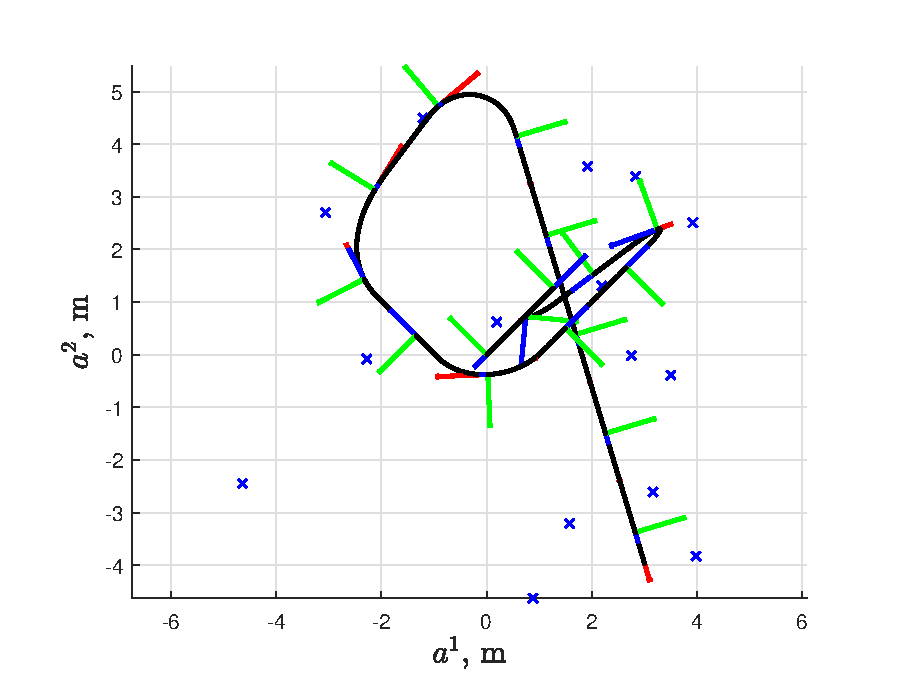
\includegraphics[width=\textwidth]{figs/traj_xy.eps} 
        \end{subfigure}
        \hfill
        \begin{subfigure}[b]{0.495\textwidth}  
            \centering 
            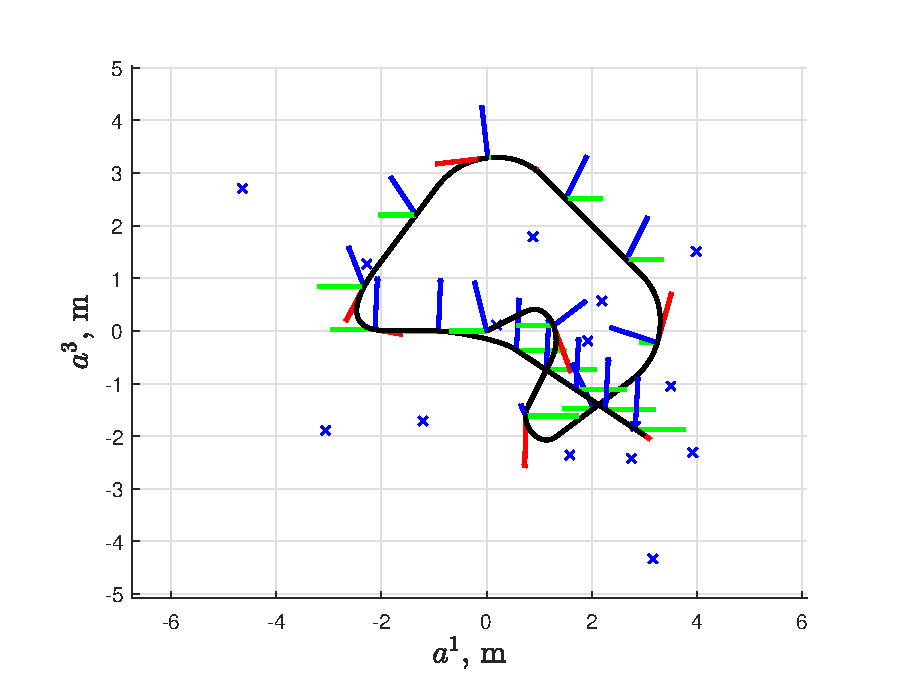
\includegraphics[width=\textwidth]{figs/traj_xz.eps} 
        \end{subfigure}
        \vskip\baselineskip
        \begin{subfigure}[b]{0.495\textwidth}   
            \centering 
            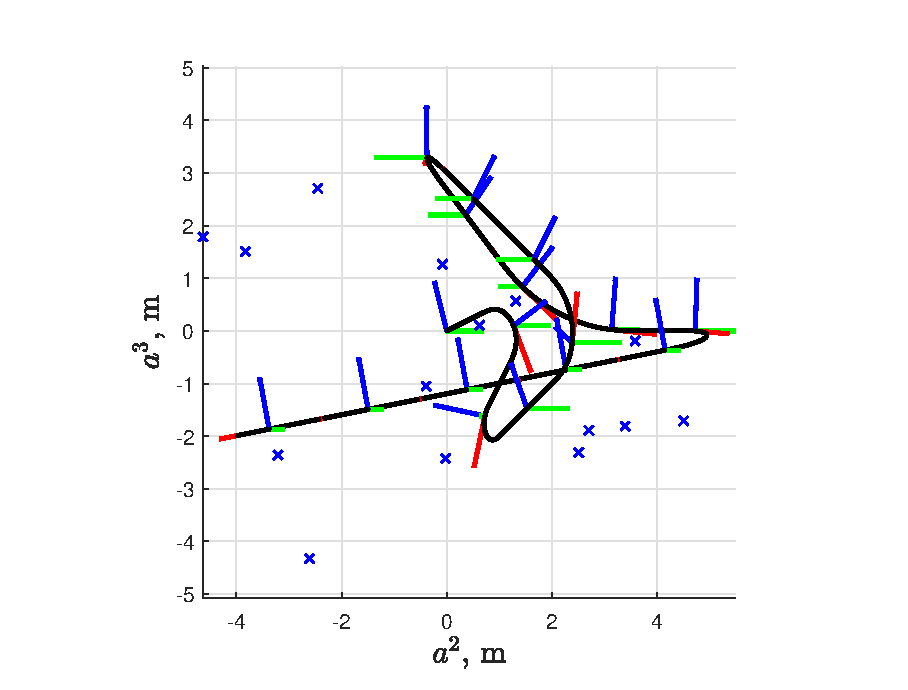
\includegraphics[width=\textwidth]{figs/traj_yz.eps}  
        \end{subfigure}
        \hfill
        \begin{subfigure}[b]{0.495\textwidth}   
            \centering 
            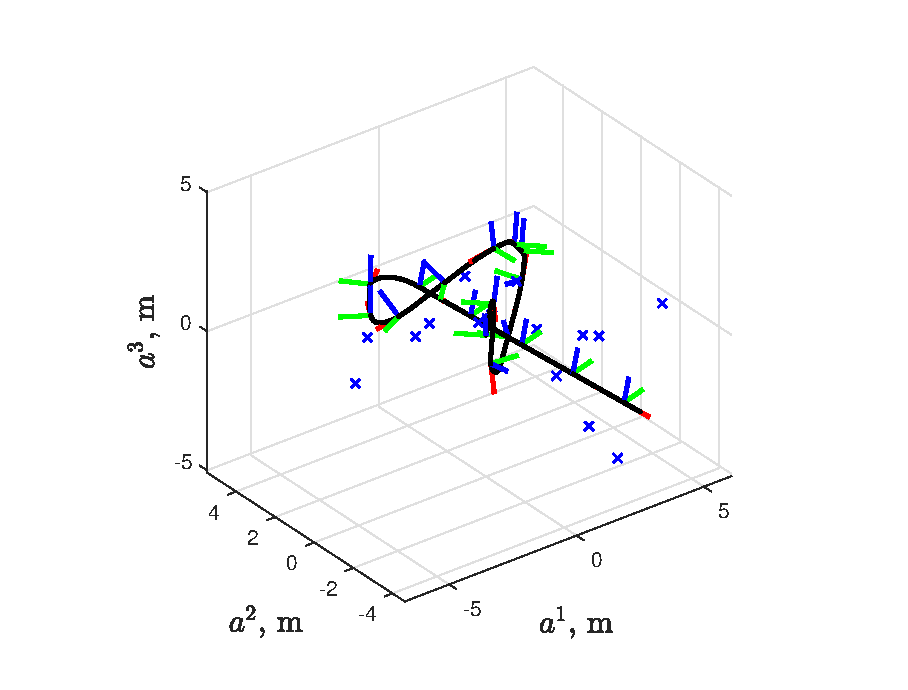
\includegraphics[width=\textwidth]{figs/traj.eps} 
        \end{subfigure} 
	\caption[Trajectory used in simulations.]{Trajectory used in simulations. The blue markers represent the landmarks, the trajectory is shown in black, and a triad is used to show the orientation at various times during the trajectory.}
	\label{fig:se3_traj}
\end{figure}

\subsubsection{Initialization}

To run appropriate Monte Carlo trials, a discussion of the initial error is necessary. When testing any EKF variant using Monte Carlo trials, the initial error $\mbfdel{x}_0$ is drawn from a normal distribution with zero mean and covariance $\mbf{P}_0$. That is, $\mbfdel{x}_0 \sim \mathcal{N}(\mbf{0},\mbf{P}_0)$. This initial error, along with the truth data, is then used to initialize the filters. For the MEKF-R and MEKF-L, this means
\begin{align*}
	\mbfhat{r}_a^{z_0w} &= \mbf{r}_a^{z_0w} - \mbfdel{r}_0, \\
	\mbfhat{C}_{ab_0} &= \mbf{C}_{ab_0}\mbfdel{C}_0^\trans. 
\end{align*}
For the LIEKF, 
\bdis
	\mbfhat{T}_0 = \mbf{T}_0\mbfdel{T}_0,    
\edis
where $\mbfdel{T}_0 = \expmapw{\mbsdel{\xi}_0}$. Similarly, for the RIEKF,
\bdis
	\mbfhat{T}_0 = \mbfdel{T}_0\mbf{T}_0.  
\edis
By using the appropriate error definition to initialize each filter, the same initial error leads to different actual initial conditions. This should not, in theory, change the difficulty of the estimation problem. Nonetheless, the effect of these differing initial conditions is tested. 

To determine the effect of changing the initial error definition, 50 Monte Carlo trials are run using two different ways of initializing the invariant filters. First, the invariant filters are initialized in a manner consistent with their error definition. They are then initialized in the same manner as the MEKF. The sensor noise standard deviations were set to $\sigma_k^1 = \SI{0.05}{rad/s}$, $\sigma_k^2 = \SI{0.05}{m/s}$ and $\sigma_k^\mathrm{R} = \SI{0.05}{\metre}$. The initial errors are drawn from a normal distribution with covariance $\mbf{P}_0 = \mathrm{diag}\left(0.1^2 \mbf{1}, \left(\f{\pi}{4}\right)^2\mbf{1}\right)$, with appropriate units. 

\sloppy The results obtained from initializing the filters in different manners are shown in Table~\ref{tab:se3_mc_err}. In practice, it is preferable to know the error in position and error in attitude separately, rather than the error in the pose. Therefore, it may be more representative to compare the filters using the MEKF error definitions. Thus, unless otherwise specified, the attitude error at each time step is given by	$\delta \phi_k = \log_{SO(3)} \left(\mbfhat{C}_{ab_k}^\trans\mbf{C}_{ab_k} \right)^\vee$ and the position error is $\delta r_k = \norm{\mbf{r}_a^{z_kw} - \mbfhat{r}_a^{z_kw}}$. Using this metric, the initialization technique does not have a significant effect on the performance of the filters. For the LIEKF, changing from the correct initialization to the MEKF initialization sees a slight increase in mean root mean square error (RMSE) for both position and attitude. The difference for the RIEKF is negligible. Importantly, independent of the way the invariant filters are initialized, they still outperform the MEKFs. In this thesis, the appropriate error definition is used to initialize the filters. In fact, doing so ensures that the initial covariance is actually representative of the initial uncertainty in the state estimate, meaning the filters are always consistent to begin the simulation.
\begin{table}[]
\centering
\begin{tabular}{|l|l|l|}
\hline
Filter             & Mean Attitude RMSE (\si{rad}) & Mean Position RMSE (\si{m}) \\ \hhline{|=|=|=|}
MEKF-L             & 0.2035             & 0.0310             \\ \hline
LIEKF - App. Init. & 0.1993             & 0.0288             \\ \hline
LIEKF - MEKF Init. & 0.2017             & 0.0297             \\ \hline
MEKF-R             & 0.0739             & 0.0532             \\ \hline
RIEKF - App. Init. & 0.0734             & 0.0475             \\ \hline
RIEKF - MEKF Init. & 0.0733             & 0.0473             \\ \hline
\end{tabular}
\caption[Results comparing different Monte Carlo initialization methods.]{Mean RMSE in the estimated states over 50 Monte Carlo simulations. The LIEKF and RIEKF were initialized both using an appropriate error definition consistent with the left and right-invariant erros and the error definition used to initialize the MEKFs.}
\label{tab:se3_mc_err}
\end{table}

\subsubsection{Monte Carlo Results}

Having determined the appropriate procedure for comparing the filters, they can be extensively tested to determine the effect of sensor noise on their performance. To do so, the noise in each sensor is varied independently. Four different trials are run. The standard deviations of the noises injected into each measurement for each trial are summarized in Table~\ref{tab:se3_noises}. When the sensor noise is varied, it is incremented by 0.05. At each noise level, 50 Monte Carlo trials are run, where the initial state estimate error and the noise profile is varied.  As in the previous simulations, the initial errors are drawn from a normal distribution with covariance $\mbf{P}_0 = \mathrm{diag}\left(0.1^2 \mbf{1}, \left(\f{\pi}{4}\right)^2\mbf{1}\right)$, with appropriate units. 

\begin{table}[]
\centering
\begin{tabular}{|l|l|l|l|}
\hline
Trial                                            & $\sigma_k^1$ (rad/s)          & $\sigma_k^2$ (m/s)            & $\sigma_k^\textrm{R}$ (m)      \\ \hhline{|=|=|=|=|}
\multicolumn{1}{|l|}{Rate Gyro Noise}            & \multicolumn{1}{l|}{0 to 1} & \multicolumn{1}{l|}{0.05}     & \multicolumn{1}{l|}{0.05}      \\ \hline
\multicolumn{1}{|l|}{Velocity Sensor Noise}      & \multicolumn{1}{l|}{0.05}     & \multicolumn{1}{l|}{0 to 1} & \multicolumn{1}{l|}{0.05}      \\ \hline
\multicolumn{1}{|l|}{Exteroceptive Sensor Noise} & \multicolumn{1}{l|}{0.05}     & \multicolumn{1}{l|}{0.05}     & \multicolumn{1}{l|}{0 to 1} \\ \hline
\multicolumn{1}{|l|}{All Noises}                 & \multicolumn{1}{l|}{0 to 1} & \multicolumn{1}{l|}{0 to 1} & \multicolumn{1}{l|}{0 to 1}  \\ \hline
\end{tabular}
\caption{Standard deviation of the noise injected into each measurement for each trial.}
\label{tab:se3_noises}
\end{table}

The results from varying the noise in the gyro, velocity sensor, correcting sensor, and all the sensors simultaneously can be found in Figures~\ref{fig:comp_noise_gyro_L}~to~\ref{fig:comp_noise_all_R}. 
Each figure presents the mean RMSE at each noise level for the IEKF and MEKF. The shaded areas encompass 80\% of the data, to show the spread of the results. The difference between the mean MEKF and IEKF RMSE is also shown. A positive value indicates that the IEKF outperformed the MEKF. The shaded area once again represents 80\% of the data. A convincing result would see the shaded area be entirely positive, meaning that only on rare occasions did the MEKF outperform the IEKF. 
On average, the invariant filters outperformed the standard MEKF in all the trials. A few important trends to note are as follows.
\begin{itemize}
	\item The increased noise magnitude had a relatively small impact on the MEKF-R and RIEKF, meaning the difference in the filters remained somewhat constant over the all the trials.
	\item Increasing the noise in the velocity sensor led to erratic behaviour of the MEKF-L, leading to some outliers.
	\item Increasing the noise in the GPS measurements led to an increase in the difference between the LIEKF and MEKF-L, as seen in Figure~\ref{fig:comp_noise_corr_L}.
\end{itemize}
It is unsurprising that the IEKF would outperform the MEKF. The state-independent Jacobians mean the computed Kalman gain is accurate, as all the matrices used in its computations are known or are made up of noise-corrupted measurements, except for the error covariance $\mbf{P}$. However, at steady state, the state estimate should be close enough to the true state that the state-dependence of the Jacobians is mitigated. This means that the improvement of the IEKF over the MEKF may simply be due to better performance in the transient. This is investigated in the next section.

%The LIEKF process model Jacobian $\mbf{A}$ depends on the velocity and rate gyro measurements. The MEKF-L process model Jacobian $\mbf{A}$ also depends on the measurement,but also on the attitude estimate $\mbfhat{C}_{ab}$. Their measurement model Jacobian $\mbf{H}$ is identical, and independent of the state. Therefore, if there is any advantage in using the LIEKF, it should manifest itself in a scenario where the attitude estimate is poor and the noise in the interoceptive sensors is low. 
%
%The RIEKF process model Jacobian $\mbf{A}$ is $\mbf{0}$, while the MEKF-R process model Jacobian $\mbf{A}$ depends on both the attitude estimate and the interoceptive measurements. This trend is continued in the measurement model Jacobians. The measurement model Jacobian for the RIEKF depends only on the known landmark position, while it depends on the state estimate for the MEKF-R. The only state dependent Jacobian in the RIEKF is $\mbf{L}$. However, the effect of this state dependency could be dampened by tuning the $\mbf{Q}_k$ matrix. 

\begin{figure}
	\centering
	\begin{subfigure}[b]{0.5\textwidth}
		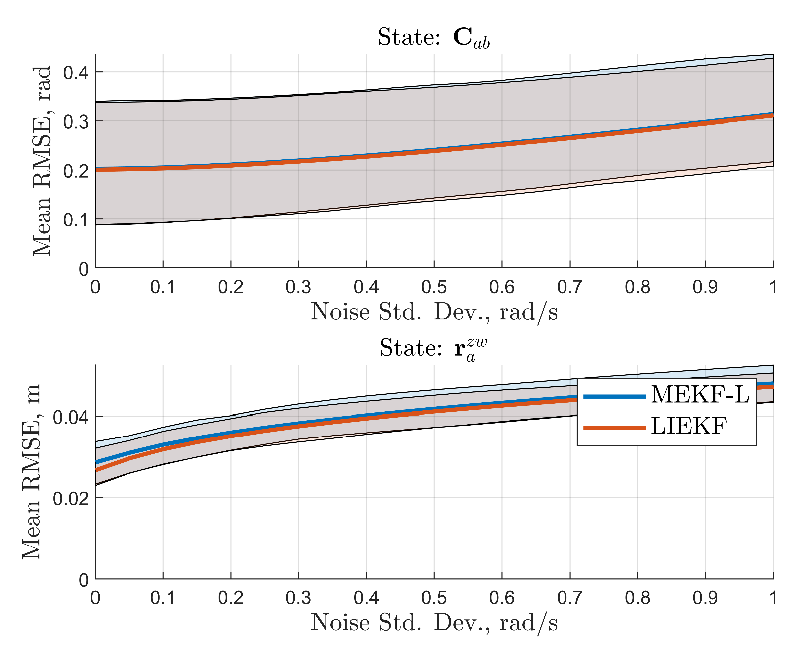
\includegraphics[width=\textwidth]{figs/se3/noise_trials/comp_noise_rmse_state_Gyro_L.eps}
		\caption{Mean RMSE for each state.}
		\label{fig:comp_noise_gyro_L_rmse}
	\end{subfigure}
	~
	\begin{subfigure}[b]{0.5\textwidth}
		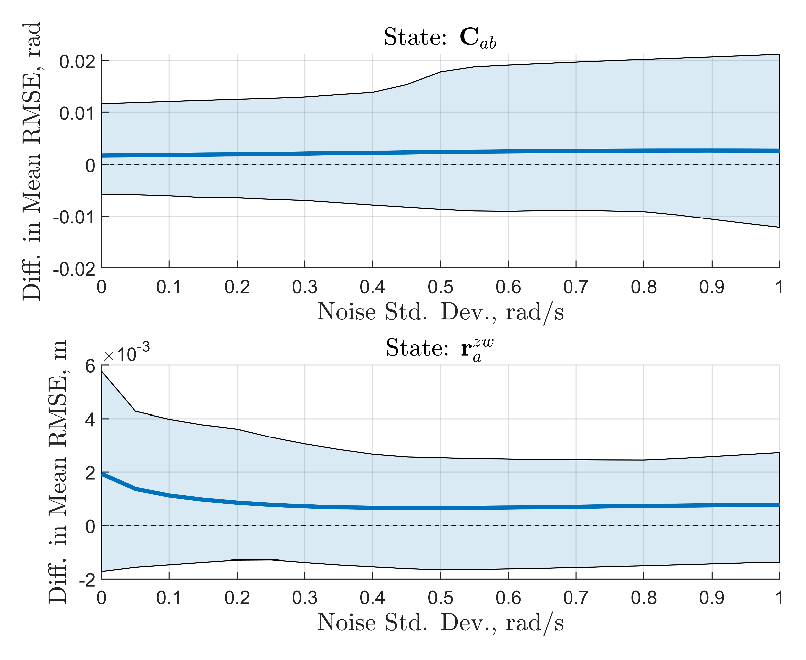
\includegraphics[width=\textwidth]{figs/se3/noise_trials/comp_noise_diff_state_Gyro_L.eps}
		\caption{Difference between in RMSE of MEKF-L and LIEKF.}
		\label{fig:comp_noise_gyro_L_diff}
	\end{subfigure}
	\caption[Results comparing the MEKF-L and LIEKF varying rate gyro noise.]{Results of 50 Monte Carlo simulations comparing the MEKF-L and LIEKF, where the amplitude of the noise in the rate gyro sensor was varied. }
	\label{fig:comp_noise_gyro_L}
\end{figure}

\begin{figure}
	\centering
	\begin{subfigure}[b]{0.5\textwidth}
		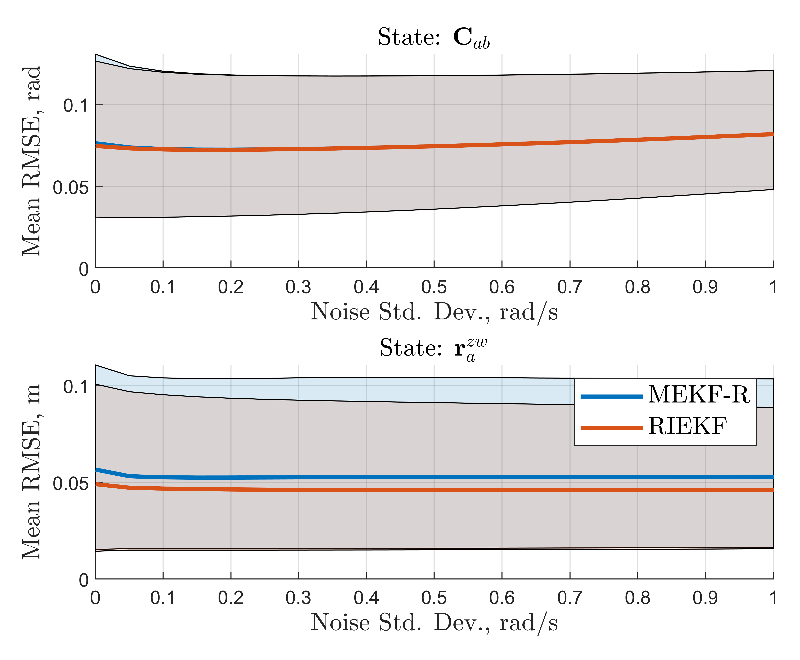
\includegraphics[width=\textwidth]{figs/se3/noise_trials/comp_noise_rmse_state_Gyro_R.eps}
		\caption{Mean RMSE for each state. }
		\label{fig:comp_noise_gyro_R_rmse}
	\end{subfigure}
	~
	\begin{subfigure}[b]{0.5\textwidth}
		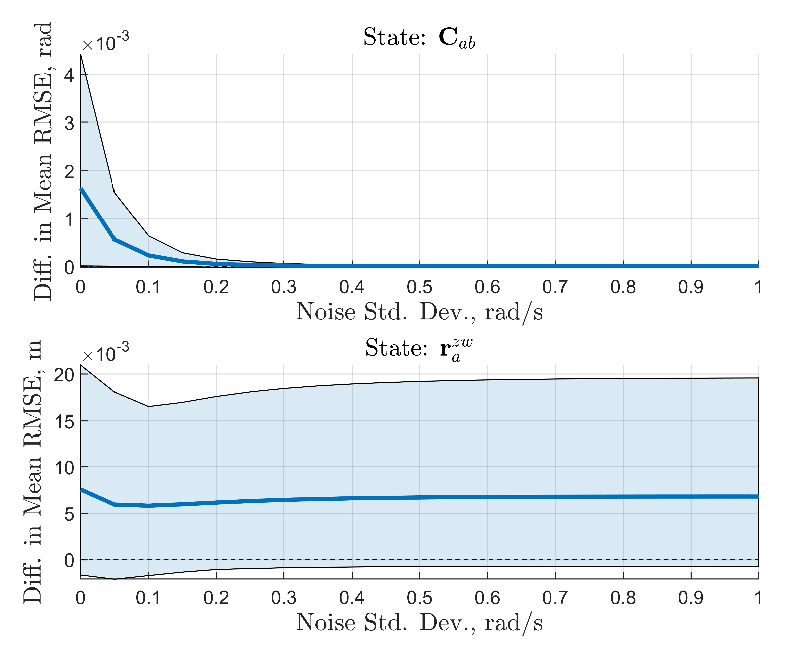
\includegraphics[width=\textwidth]{figs/se3/noise_trials/comp_noise_diff_state_Gyro_R.eps}
		\caption{Difference in RMSE between MEKF-R and RIEKF.}
		\label{fig:comp_noise_gyro_R_diff}
	\end{subfigure}
	\caption[Results comparing the MEKF-R and RIEKF varying rate gyro noise.]{Results of 50 Monte Carlo simulations comparing the MEKF-R and RIEKF, where the amplitude of the noise in the rate gyro sensor was varied. }
	\label{fig:comp_noise_gyro_R}
\end{figure}
% Velocity
\begin{figure}
	\centering
	\begin{subfigure}[b]{0.5\textwidth}
		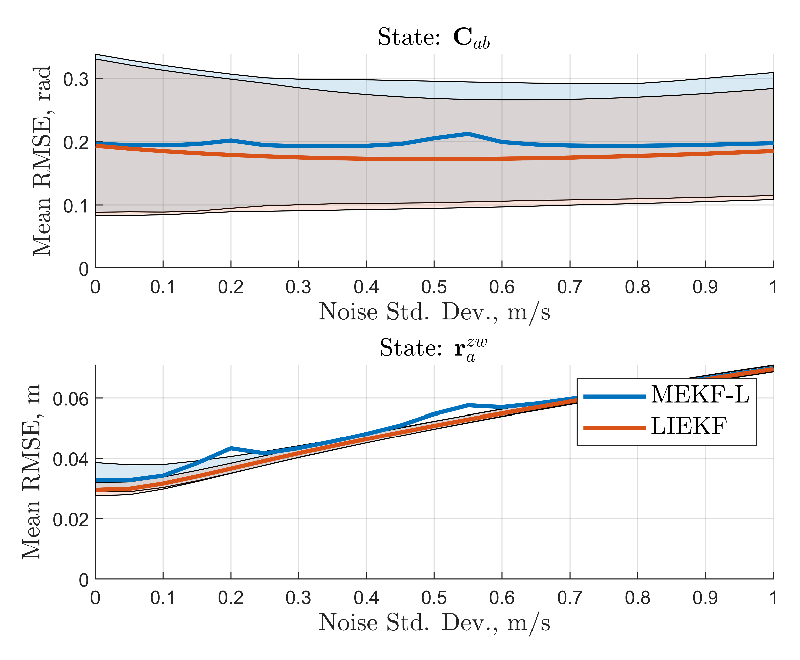
\includegraphics[width=\textwidth]{figs/se3/noise_trials/comp_noise_rmse_state_Vel_L.eps}
		\caption{Mean RMSE for each state.}
	\end{subfigure}
	~
	\begin{subfigure}[b]{0.5\textwidth}
		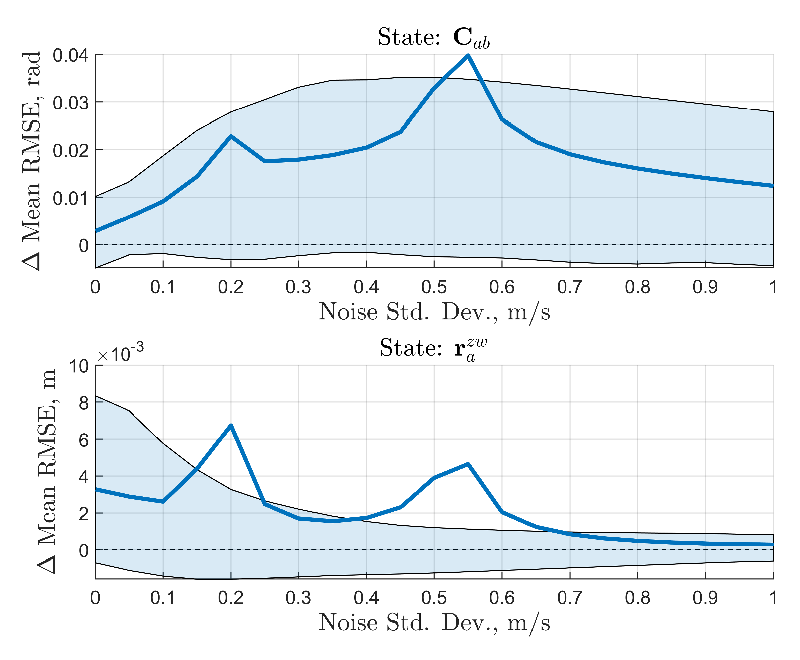
\includegraphics[width=\textwidth]{figs/se3/noise_trials/comp_noise_diff_state_Vel_L.eps}
		\caption{Difference between in RMSE of MEKF-L and LIEKF.}
	\end{subfigure}
	\caption[Results comparing the MEKF-L and LIEKF varying velocity sensor noise.]{Results of 50 Monte Carlo simulations comparing the MEKF-L and LIEKF, where the amplitude of the noise in the velocity sensor was varied. }
	\label{fig:comp_noise_vel_L}
\end{figure}


\begin{figure}
	\centering
	\begin{subfigure}[b]{0.5\textwidth}
		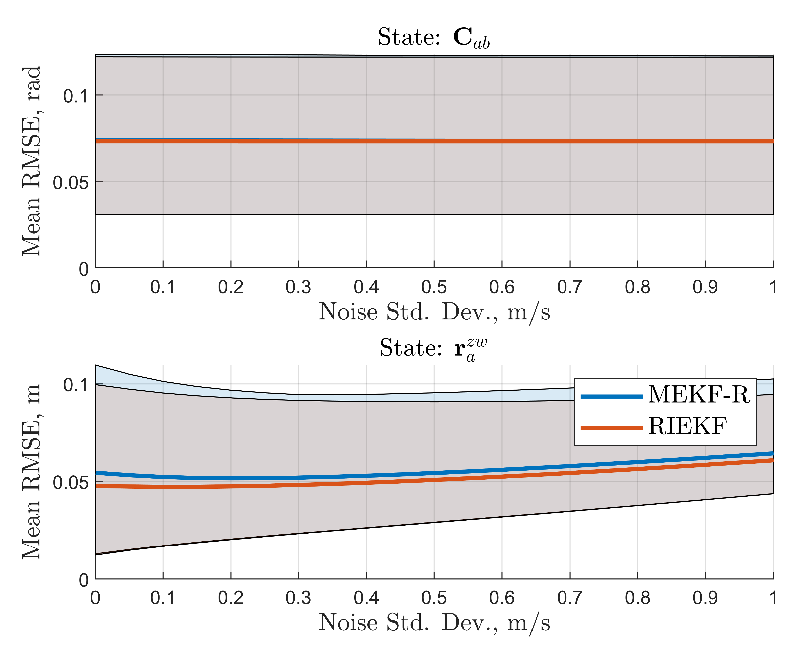
\includegraphics[width=\textwidth]{figs/se3/noise_trials/comp_noise_rmse_state_Vel_R.eps}
		\caption{Mean RMSE for each state.}
	\end{subfigure}
	~
	\begin{subfigure}[b]{0.5\textwidth}
		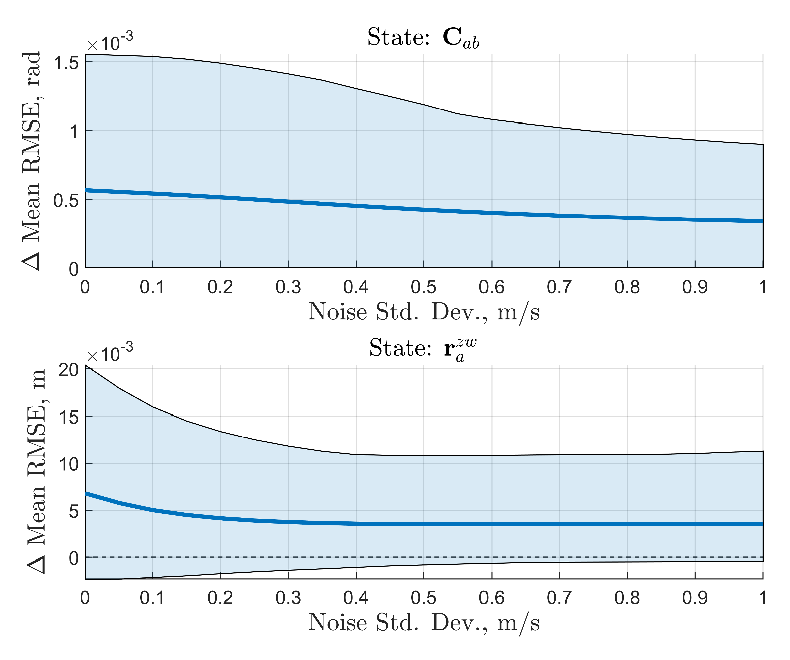
\includegraphics[width=\textwidth]{figs/se3/noise_trials/comp_noise_diff_state_Vel_R.eps}
		\caption{Difference between in RMSE of MEKF-R and RIEKF.}
	\end{subfigure}
	\caption[Results comparing the MEKF-R and RIEKF varying velocity sensor noise.]{Results of 50 Monte Carlo simulations comparing the MEKF-R and RIEKF, where the amplitude of the noise in the velocity sensor was varied. }
	\label{fig:comp_noise_vel_R}
\end{figure}

\begin{figure}
	\centering
	\begin{subfigure}[b]{0.5\textwidth}
		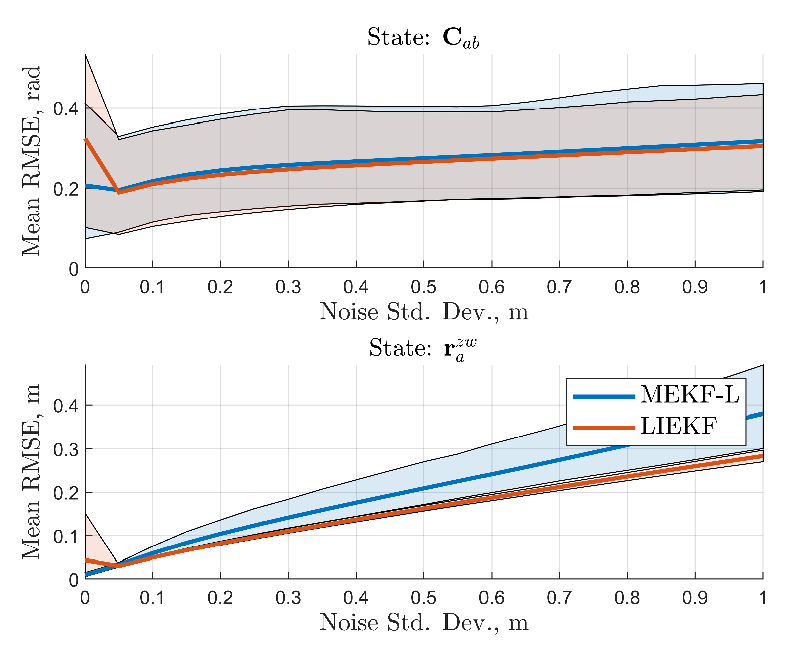
\includegraphics[width=\textwidth]{figs/se3/noise_trials/comp_noise_rmse_state_Corr_L.eps}
		\caption{Mean RMSE for each state.}
	\end{subfigure}
	~
	\begin{subfigure}[b]{0.5\textwidth}
		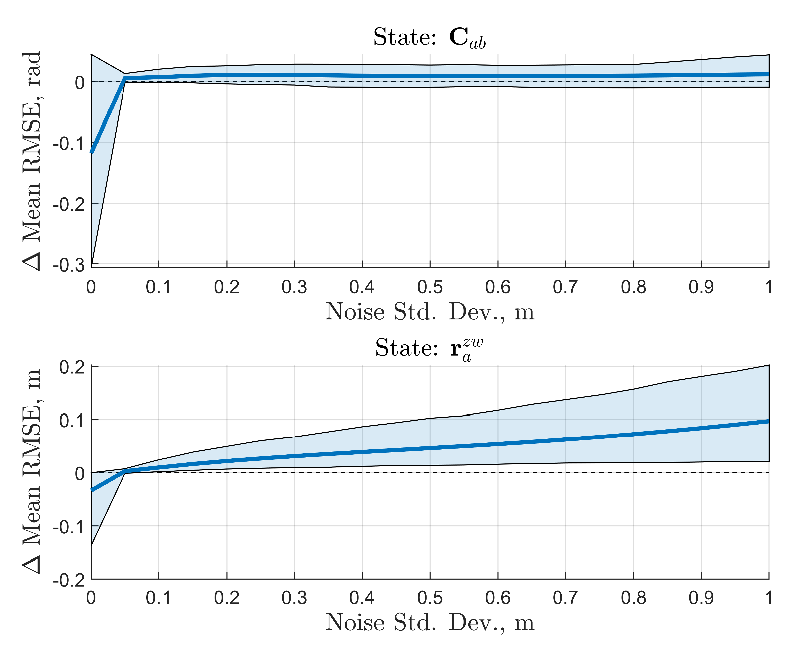
\includegraphics[width=\textwidth]{figs/se3/noise_trials/comp_noise_diff_state_Corr_L.eps}
		\caption{Difference in mean RMSE of MEKF-L and LIEKF.}
	\end{subfigure}
	\caption[Results comparing the MEKF-L and LIEKF varying correcting sensor noise.]{Results of 50 Monte Carlo simulations comparing the MEKF-L and LIEKF, where the amplitude of the noise in the correcting sensor was varied. }
	\label{fig:comp_noise_corr_L}
\end{figure}


\begin{figure}
	\centering
	\begin{subfigure}[b]{0.5\textwidth}
		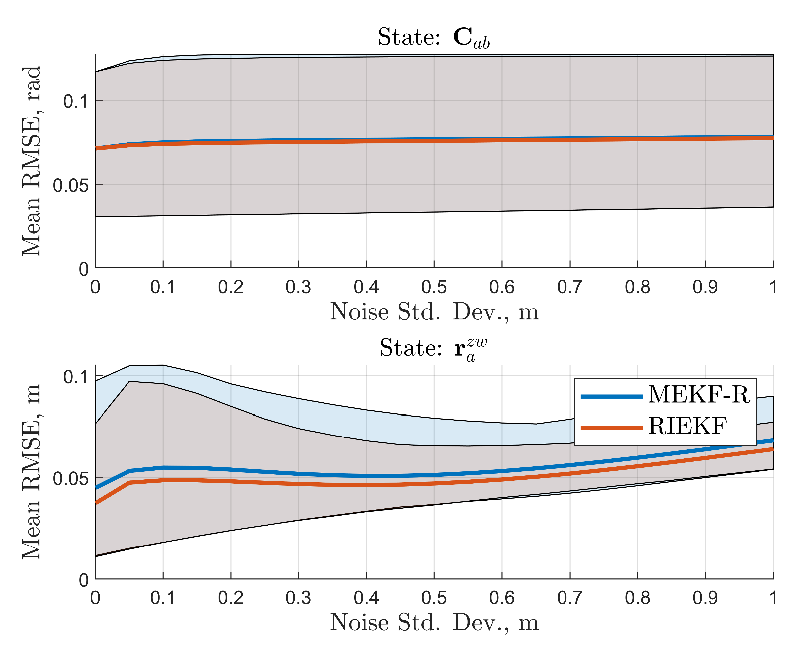
\includegraphics[width=\textwidth]{figs/se3/noise_trials/comp_noise_rmse_state_Corr_R.eps}
		\caption{Mean RMSE for each state.}
	\end{subfigure}
	~
	\begin{subfigure}[b]{0.5\textwidth}
		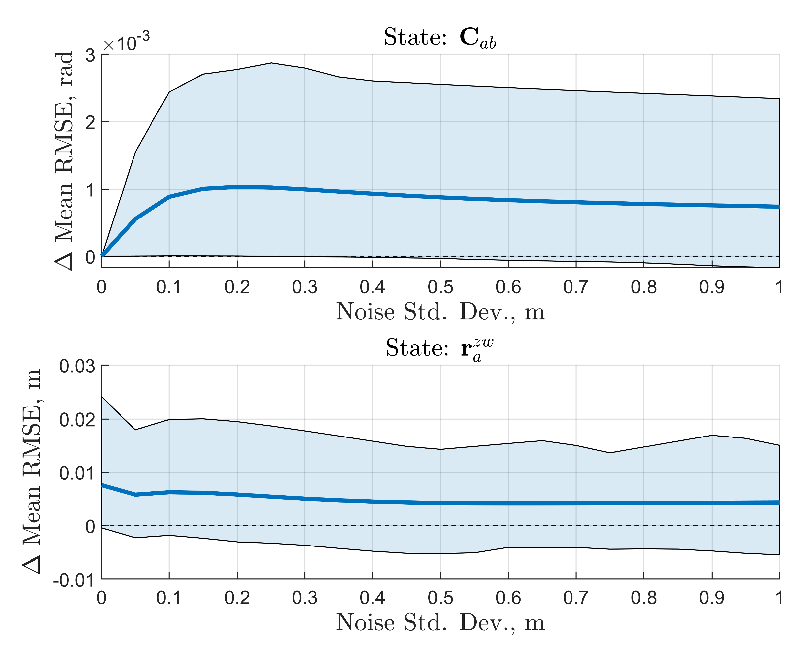
\includegraphics[width=\textwidth]{figs/se3/noise_trials/comp_noise_diff_state_Corr_R.eps}
		\caption{Difference in mean RMSE of MEKF-R and RIEKF.}
	\end{subfigure}
	\caption[Results comparing the MEKF-R and RIEKF varying correcting sensor noise.]{Results of 50 Monte Carlo simulations comparing the MEKF-R and RIEKF, where the amplitude of the noise in the correcting sensor was varied. }
	\label{fig:comp_noise_corr_R}
\end{figure}

% All
\begin{figure}
	\centering
	\begin{subfigure}[b]{0.5\textwidth}
		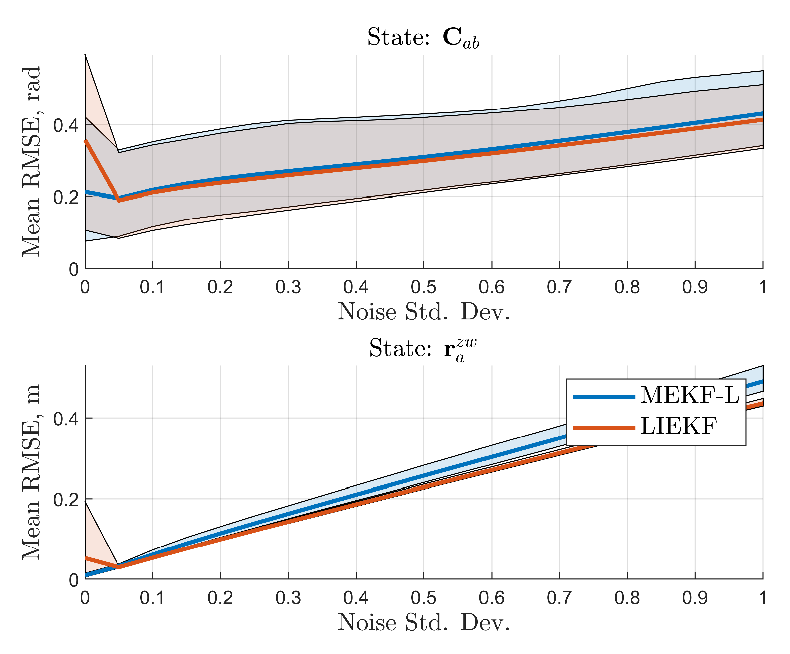
\includegraphics[width=\textwidth]{figs/se3/noise_trials/comp_noise_rmse_state_All_L.eps}
		\caption{Mean RMSE for each state.}
	\end{subfigure}
	~
	\begin{subfigure}[b]{0.5\textwidth}
		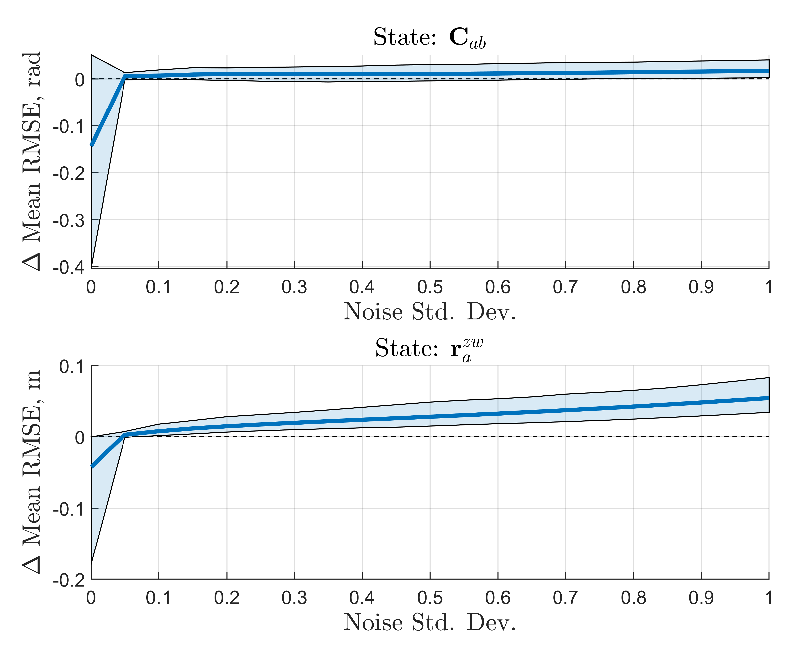
\includegraphics[width=\textwidth]{figs/se3/noise_trials/comp_noise_diff_state_All_L.eps}
		\caption{Difference in mean RMSE of MEKF-L and LIEKF.}
	\end{subfigure}
	\caption[Results comparing the MEKF-L and LIEKF varying all sensor noise.]{Results of 50 Monte Carlo simulations comparing the MEKF-L and LIEKF, where the amplitude of the noise in all sensors was varied. }
	\label{fig:comp_noise_all_L}
\end{figure}

\begin{figure}
	\centering
	\begin{subfigure}[b]{0.5\textwidth}
		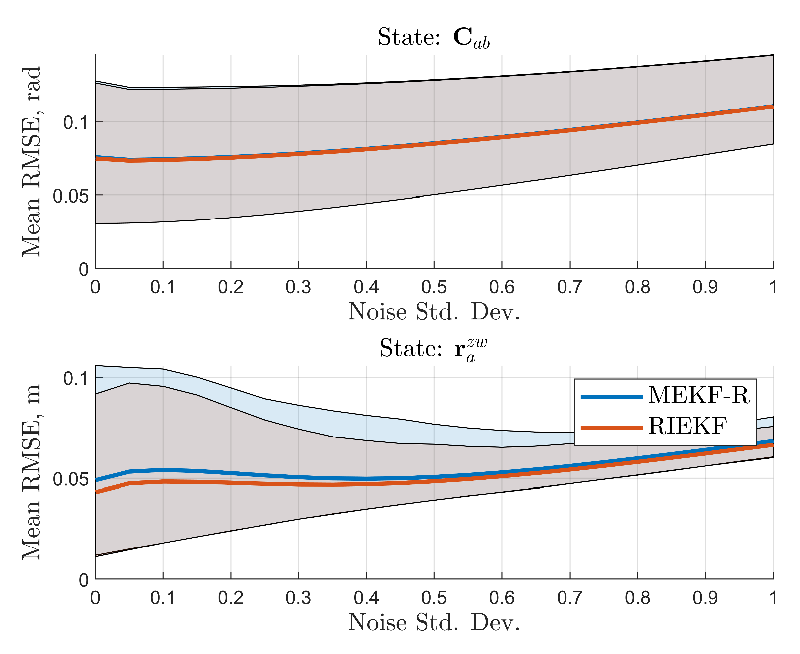
\includegraphics[width=\textwidth]{figs/se3/noise_trials/comp_noise_rmse_state_All_R.eps}
		\caption{Mean RMSE for each state.}
	\end{subfigure}
	~
	\begin{subfigure}[b]{0.5\textwidth}
		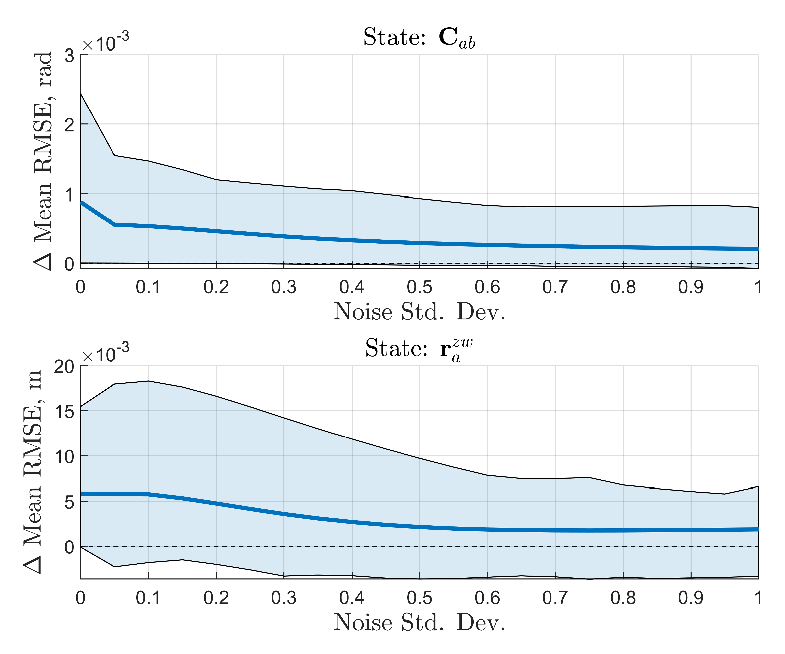
\includegraphics[width=\textwidth]{figs/se3/noise_trials/comp_noise_diff_state_All_R.eps}
		\caption{Difference in mean RMSE of MEKF-R and RIEKF.}
	\end{subfigure}
	\caption[Results comparing the MEKF-R and RIEKF varying all sensor noise.]{Results of 50 Monte Carlo simulations comparing the MEKF-R and RIEKF, where the amplitude of the noise in all sensors was varied. }
	\label{fig:comp_noise_all_R}
\end{figure}

\FloatBarrier

\subsubsection{Effect of Initial Attitude Error}

As discussed in \cite{Barrau2017} and \cite{Barrau2018}, the main advantage the IEKF claims over the MEKF are its convergence properties. Therefore, it may be reasonable to expect the IEKFs to perform substantially better than the MEKFs for high initial error. To test this, $\delta \phi_3$ was varied from 0 \si{\radian} to $\f{23\pi}{24}$ \si{\radian} in increments of \SI{\pi/24}{\radian}. In degrees, $\delta \phi_3$ is varied from  \SI{0}{\degree} to \SI{172.5}{\degree} in increments of \SI{7.5}{\degree}. The initial position was initialized such that there was zero initial error. 

The magnitude of the standard deviation of the noise in the sensors are set to $\sigma_k^1 = \SI{0.05}{rad/s}$, $\sigma_k^2 = \SI{0.05}{m/s}$ and $\sigma_k^\mathrm{R} = \SI{0.05}{m}$. The initial covariance is set $\mbf{P}_0 = \mathrm{diag}(\delta \phi_3^2\mbf{1},1 \times 10^{-4}\mbf{1})$, with appropriate units. This was chosen to reflect the varying uncertainty in the initial attitude and high certainty in the initial position. At each initial attitude error, 50 trials were run, where the noise profile was varied. The results of these simulations are shown in Figure~\ref{fig:comp_att}. The results comparing the RIEKF and MEKF-R show that at high initial attitude, error, the RIEKF consistently outperforms the MEKF-R. This is especially the case for position. The improvement in attitude error is marginal. The trend is less clear when comparing the LIEKF and MEFK-L, but the conclusion is similar. As expected, when the initial estimate of the state is poor, the invariant filters offer superior performance.  When the initial state estimate is accurate, the Jacobians are close to the true Jacobians, nullifying any advantage the IEKFs had over the MEKFs, and their performance is indistinguishable.
\begin{figure}
	\centering
	\begin{subfigure}[b]{0.5\textwidth}
		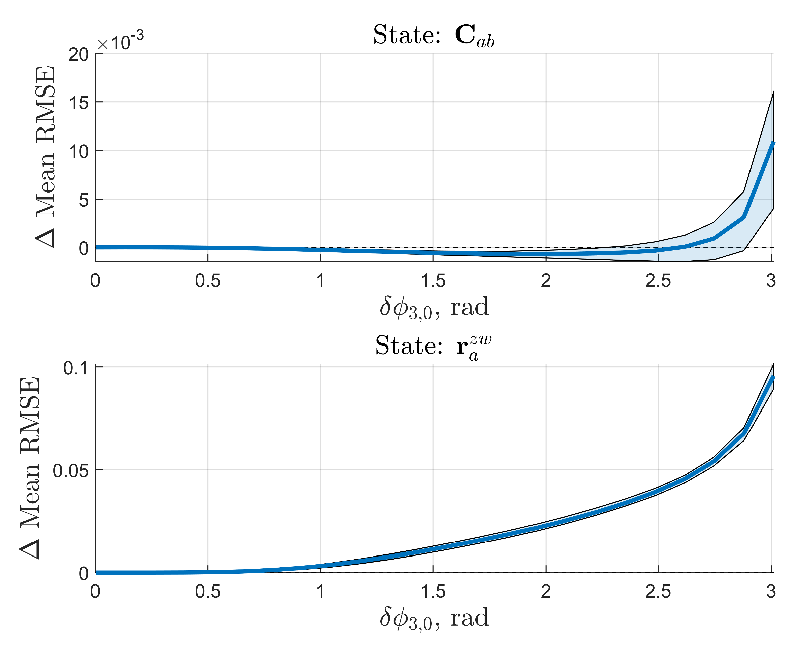
\includegraphics[width=\textwidth]{figs/se3/noise_trials/comp_att_diff_state_Att_R.eps}
		\caption{MEKF-R and RIEKF Comparison.}
	\end{subfigure}
	~
	\begin{subfigure}[b]{0.5\textwidth}
		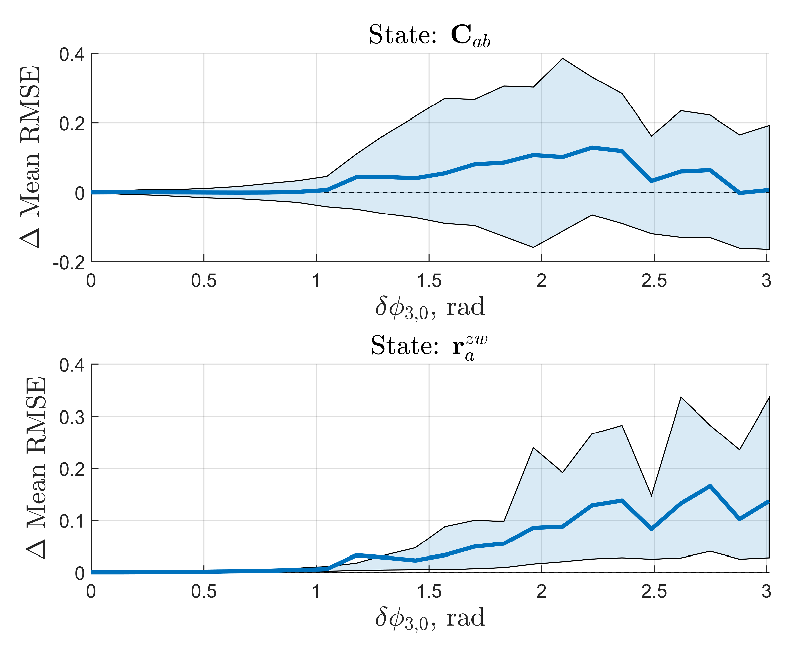
\includegraphics[width=\textwidth]{figs/se3/noise_trials/comp_att_diff_state_Att_L.eps}
		\caption{MEKF-L and LIEKF Comparison.}
	\end{subfigure}
	\caption[Results of different noise profiles where $\delta \phi_3$ was varied.]{Results of 50 different noise profiles comparing invariant and multiplicative filters, where $\delta \phi_3$ was varied. }
	\label{fig:comp_att}
\end{figure}

\FloatBarrier

\section{Applying the IEKF to a Realistic Data Set}
\label{sec:se3_real_data}

The measurement model used in Section~\ref{ssec:SE3_RIEKF} is perfectly right-invariant. However, this is not a realistic measurement model, as no sensor exists that directly measures a relative landmark position. Rather, a LIDAR or camera is used. These measurements are neither left nor right-invariant. Therefore, the IEKF can not be directly applied, and must be adapted, as demonstrated in \cite{Barrau2015aa} with a range-and-bearing measurement model. To illustrate this, the sample problem from the previous section is replicated using a camera as an exteroceptive sensor. Let point $c$ be fixed to the camera, and frame $\rframe{c}$ rotate with the camera. The position of the $i^{th}$ landmark $p^i$ relative to $c$ resolved in the camera frame is 
\beq
	\mbf{r}_{c}^{p_ic} = \mbf{C}_{bc}^\trans(\mbf{C}_{ab}^\trans(\mbf{r}_a^{p_iw} - \mbf{r}_a^{zw}) - \mbf{r}_b^{cz}), \label{eq:se3_real_meas_1}
\eeq
where $\mbf{C}_{bc}$ and $\mbf{r}_b^{cz}$ are known. Letting $\mbf{r}_c^{p_ic} = [ \; x^i \; y^i \; z^i \; ]^\trans$, the measurements from a stereo camera at time $t_k$ are then \cite[p. 208]{Barfoot2017}
\beq
	\mbf{y}_k^i = \mbf{g}(\mbf{r}_{c_k}^{p_ic_k}) =  \f{1}{z_k^i}
	\bma{c}
		f_u x_k^i \\
		f_v y_k^i \\ 
		f_u (x_k^i - b) \\
		f_v y_k^i
	\ema
	+
	\bma{c}
		c_u \\
		c_v \\ 
		c_u \\
		c_v 
	\ema + \mbf{v}_k\label{eq:se3_real_meas}
\eeq
where $c_u$ and $c_v$ are the horizontal and vertical optical centres of the camera in pixels, $f_u$ and $f_v$ are the horizontal and vertical focal lengths of the camera in pixels, and $b$ is the distance between the two centers of projection of the camera, in meters. The noise $\mbf{v}_k \sim \mc{N}(\mbf{0},\mbf{R}_k)$ is zero-mean white noise with covariance $\mbf{R}_k$. 

\subsection{Right-Invariant Kalman Filter Derivation}

As the measurement model \eqref{eq:se3_real_meas} is a function of a right-invariant measurement \eqref{eq:se3_real_meas_1}, a RIEKF is implemented. Therefore, the process model Jacobians from Section~\ref{ssec:SE3_RIEKF} are kept. Typically, the innovation $\mbf{z}_k^i = \mbfch{T}_k(\mbf{y}_k^i - \mbfch{y}_k^i)$ would be linearized to obtain the measurement model Jacobians. However, this is impossible to do in this case, as it is impossible to multiply the measurement from the camera by an element of $SE(3)$.  To avoid this, the standard innovation from the EKF, $\mbf{z}_k^i = \mbf{y}_k^i - \mbfch{y}_k^i$, must be used. 

To compute the new measurement model Jacobians, consider the first-order Taylor series expansion of \eqref{eq:se3_real_meas},
\bdis
	\mbfch{y}_k^i + \mbfdel{y}_k^i =  \mbf{g}(\mbfch{r}_{c_k}^{p_ic_k}) + \underbrace{\left.\f{\partial \mbf{g}(\mbf{r}_{c_k}^{p_ic_k})}{\partial \mbf{x}_k}\right\rvert_{\mbfch{x}_k,\mbfch{v}_k}}_{\mbf{H}_k}\mbfdel{x}_k + \underbrace{\left.\f{\partial \mbf{g}(\mbf{r}_{c_k}^{p_ic_k})}{\partial \mbf{v}_k}\right\rvert_{\mbfch{x}_k,\mbfch{v}_k}}_{\mbf{M}_k}\mbfdel{v}_k.
\edis
Using the chain rule, the matrix $\mbf{H}_k$ is
\bdis
	\mbf{H}_k = \left.\f{\partial \mbf{g}(\mbf{r}_{c_k}^{p_ic_k})}{\partial \mbf{x}_k}\right\rvert_{\mbfch{x}_k,\mbfch{v}_k} = \left.\f{\partial \mbf{g}(\mbf{r}_{c_k}^{p_ic_k})}{\partial  \mbf{r}_{c_k}^{p_ic_k}} \f{\partial  \mbf{r}_{c_k}^{p_ic_k}}{\partial \mbf{x}_k}\right\rvert_{\mbfch{x}_k,\mbfch{v}_k}.
\edis
The term $\left.\f{\partial  \mbf{r}_{c_k}^{p_ic_k}}{\partial \mbf{x}_k}\right\rvert_{\mbfch{x}_k,\mbfch{v}_k}$ is found using the perturbation method. The right-invariant error in the pose $\delta \mbfch{T}_k$ can be written as
\begin{align*}
	\delta \mbfch{T}_k &= \mbfch{T}_k\mbf{T}_k^{-1} \\
	&= 
	\bma{cc}
		\mbfch{C}_{ab_k} & \mbfch{r}_a^{z_kw} \\
		\mbf{0} & 1 
	\ema
	\bma{cc}
		\mbf{C}_{ab_k}^\trans & -\mbf{C}_{ab_k}^\trans\mbf{r}_a^{z_kw} \\
		\mbf{0} & 1 
	\ema \\
	&= 
	\bma{cc}
		\mbfch{C}_{ab_k}\mbf{C}_{ab_k}^\trans & \mbfch{C}_{ab_k}\mbf{C}_{ab_k}^\trans\mbf{r}_a^{z_kw} - \mbfch{r}_a^{z_kw} \\
		\mbf{0} & 1 
	\ema \\
	&= 
	\bma{cc}
		\delta \mbfch{C}_k & \delta \mbfch{C}_k \mbf{r}_a^{z_kw} - \mbfch{r}_a^{z_kw} \\
		\mbf{0} & 1 
	\ema \\
	&= 	
	\bma{cc}
		\delta \mbfch{C}_k & \delta \mbfch{r}_k \\
		\mbf{0} & 1 
	\ema \\
	&= 
	\bma{cc}
		\exp_{SO(3)}\left({\delta \mbsch{\xi}_k^\phi}\right) & \mbf{J}\delta\mbsch{\xi}_k^\mathrm{r} \\
		\mbf{0} & 1 
	\ema.
\end{align*}
Thus, perturbing the attitude results in $\mbf{C}_{ab_k} = \delta \mbfch{C}_k^\trans \mbfch{C}_{ab_k}$, which can also be written $\mbf{C}_{ab_k} = \exp_{SO(3)}\left(-{\delta \mbsch{\xi}_k^\phi}\right)\mbfch{C}_{ab_k}$. The position perturbation results in $\mbf{r}_a^{z_kw} = \mbfdel{C}_k^\trans(\mbfch{r}_a^{z_kw} - \mbfdel{r}_k)$, which is equivalent to $\mbf{r}_a^{z_kw} = \exp_{SO(3)}\left(-{\delta \mbsch{\xi}_k^\phi}\right)(\mbfch{r}_a^{z_kw} - \mbf{J}\delta\mbsch{\xi}_k^\mathrm{r})$. Using these perturbations, along with $\mbf{r}_{c_k}^{p_ic_k} = \mbfch{r}_{c_k}^{p_ic_k} + \mbfdel{r}_{c_k}^{p_ic_k}$, yields
\begin{align}
	\mbf{r}_{c_k}^{p_ic_k} &= \mbf{C}_{bc}^\trans(\mbf{C}_{ab_k}^\trans(\mbf{r}_a^{p_iw} - \mbf{r}_a^{z_k^iw}) - \mbf{r}_{b}^{cz}), \notag \\
	\mbfch{r}_{c_k}^{p_ic_k} + \mbfdel{r}_{c_k}^{p_ic_k} &= \mbf{C}_{bc}^\trans\bigg(\left(\exp_{SO(3)}\left(-{\delta \mbsch{\xi}_k^\phi}\right)\mbfch{C}_{ab_k}\right)^\trans \notag \\
	& \qquad \qquad \qquad \qquad \qquad \qquad \left(\mbf{r}_a^{p_iw} - \exp_{SO(3)}\left(-{\delta \mbsch{\xi}_k^\phi}\right)\left(\mbfch{r}_a^{z_kw} - \mbf{J}\delta\mbsch{\xi}_k^\mathrm{r}\right)\right) - \mbf{r}_{b}^{cz}\bigg) \notag \\ 
	 &= \mbf{C}_{bc}^\trans\left(\mbfch{C}_{ab_k}^\trans\exp_{SO(3)}\left({\delta \mbsch{\xi}_k^\phi}\right)\left(\mbf{r}_a^{p_iw} - \exp_{SO(3)}\left(-{\delta \mbsch{\xi}_k^\phi}\right)(\mbfch{r}_a^{z_kw} -  \mbf{J}\delta\mbsch{\xi}_k^\mathrm{r})\right) - \mbf{r}_{b}^{cz}\right). \label{eq:se3_real_right_1}
\end{align}
Linearizing \eqref{eq:se3_real_right_1} by letting $\exp_{SO(3)}\left(-{\delta \mbsch{\xi}_k^\phi}\right) \approx \mbf{1} + {\delta \mbsch{\xi}_k^\phi}^\times$ and $\mbf{J} \approx \mbf{1}$, 
\begin{align*}
	\mbfch{r}_{c_k}^{p_ic_k} + \mbfdel{r}_{c_k}^{p_ic_k} &= \mbf{C}_{bc}^\trans(\mbfch{C}_{ab_k}^\trans(\mbf{1} +  {\delta \mbsch{\xi}_k^\phi}^\times)(\mbf{r}_a^{p_iw} - (\mbf{1} -  {\delta \mbsch{\xi}_k^\phi}^\times)(\mbfch{r}_a^{z_kw} - \delta\mbsch{\xi}_k^\mathrm{r})) - \mbf{r}_{b}^{cz}) \\
	&= \mbf{C}_{bc}^\trans(\mbfch{C}_{ab_k}^\trans(\mbf{r}_a^{p_iw} - \mbfch{r}_a^{z_kw})  +  \mbfch{C}_{ab_k}^\trans(\delta\mbsch{\xi}_k^\mathrm{r} +  {\delta \mbsch{\xi}_k^\phi}^\times\mbfch{r}_a^{z_kw}) + \mbfch{C}_{ab_k}^\trans {\delta \mbsch{\xi}_k^\phi}^\times(\mbf{r}_a^{p_iw} - \mbfch{r}_a^{z_kw}) - \mbf{r}_{b}^{cz}), \\
	\mbfdel{r}_{c_k}^{p_ic_k} &= \mbf{C}_{bc}^\trans(\mbfch{C}_{ab_k}^\trans(\delta\mbsch{\xi}_k^\mathrm{r}  +  {\delta \mbsch{\xi}_k^\phi}^\times\mbfch{r}_a^{z_kw}) + \mbfch{C}_{ab_k}^\trans {\delta \mbsch{\xi}_k^\phi}^\times(\mbf{r}_a^{p_iw} - \mbfch{r}_a^{z_kw})) \\
	&= \mbf{C}_{bc}^\trans(\mbfch{C}_{ab_k}^\trans\delta\mbsch{\xi}_k^\mathrm{r} + \mbfch{C}_{ab_k}^\trans {\delta \mbsch{\xi}_k^\phi}^\times(\mbf{r}_a^{p_iw} - \mbfch{r}_a^{z_kw} + \mbfch{r}_a^{z_kw})) \\
	&= \mbf{C}_{bc}^\trans\mbfch{C}_{ab_k}^\trans\delta\mbsch{\xi}_k^\mathrm{r} - \mbf{C}_{bc}^\trans\mbfch{C}_{ab_k}^\trans{\mbf{r}_a^{p_iw}}^\times {\delta \mbsch{\xi}_k^\phi}.
\end{align*}
Therefore
\bdis
	\left.\f{\partial  \mbf{r}_{c_k}^{p_ic_k}}{\partial \mbf{x}_k}\right\rvert_{\mbfch{x}_k,\mbfch{v}_k} =
	\bma{cc}
		-\mbf{C}_{bc}^\trans\mbfch{C}_{ab_k}^\trans{\mbf{r}_a^{p_iw}}^\times & \mbf{C}_{bc}^\trans\mbfch{C}_{ab_k}^\trans
	\ema.
\edis
The term $\f{\partial \mbf{g}(\mbf{r}_{c_k}^{p_ic_k})}{\partial  \mbf{r}_{c_k}^{p_ic_k}}$ is computed analytically, yielding
\bdis
	\f{\partial \mbf{g}(\mbf{r}_{c_k}^{p_ic_k})}{\partial  \mbf{r}_{c_k}^{p_ic_k}} = \f{1}{z_k^i}
	\bma{ccc}
		f_u & 0 & -\f{f_u x_k^i}{z_k^i} \\
		0 & f_v & -\f{f_v y_k^i}{z_k^i} \\
		f_u & 0 & -\f{f_u (x_k^i - b)}{z_k^i} \\
		0 & f_v & -\f{f_v y_k^i}{z_k^i} \\
	\ema.
\edis
Therefore, the measurement model Jacobians are 
\beq
	\mbf{H}_k = \underset{i = 1,\ldots,m}{\textrm{row}}\left(
	\f{1}{z_k^i}
	\bma{ccc}
		f_u & 0 & -\f{f_u x_k^i}{z_k^i} \\
		0 & f_v & -\f{f_v y_k^i}{z_k^i} \\
		f_u & 0 & -\f{f_u (x_k^i - b)}{z_k^i} \\
		0 & f_v & -\f{f_v y_k^i}{z_k^i} \\
	\ema
	\bma{cc}
		-\mbf{C}_{bc}^\trans\mbfch{C}_{ab_k}^\trans{\mbf{r}_a^{p_iw}}^\times & \mbf{C}_{bc}^\trans\mbfch{C}_{ab_k}^\trans
	\ema \right) \label{eq:se3_H_real_riekf}
\eeq
and $\mbf{M} = \mbf{1}$.
Comparing \eqref{eq:se3_H_real_riekf} to \eqref{eq:se3_H_riekf}, the impacts of the using the camera model become clear. The measurement model Jacobian depends on the state estimate, as it depends on $\mbfch{r}_{c_k}^{p_ic_k}$ and $\mbfch{C}_{ab_k}$.

\subsection{MEKF Solution}

The process model Jacobians are identical to those in Section~\ref{ssec:se3_EKF}. Using a similar technique to the RIEKF just described, the measurement Jacobians for the MEKF are 
\beq
	\mbf{H}_k = \underset{i = 1,\ldots,m}{\textrm{row}}\left\{
	\f{1}{z_k^i}
	\bma{ccc}
		f_u & 0 & -\f{f_u x_k^i}{z_k^i} \\
		0 & f_v & -\f{f_v y_k^i}{z_k^i} \\
		f_u & 0 & -\f{f_u (x_k^i - b)}{z_k^i} \\
		0 & f_v & -\f{f_v y_k^i}{z_k^i} \\
	\ema
	\bma{cc}
		\mbf{C}_{bc}^\trans\left(\mbfch{C}_{ab_k}^\trans(\mbf{r}_a^{p_iw} - \mbfch{r}_a^{z_k w})\right)^\times & -\mbf{C}_{bc}^\trans\mbfch{C}_{ab_k}^\trans
	\ema \right\} \label{eq:se3_H_real_ekf}
\eeq
and $\mbf{M} = \mbf{1}$.

\subsection{Filtering Using Pseudo-measurements}

To avoid the state-dependent $\mbf{H}_k$ matrix from the previous section, the measurement model must be right-invariant. To attain this using the nonlinear camera model, the measurements are preprocessed so that the output of the sensor is $\mbf{r}_{b_k}^{p_iz_k}$.  The issue with doing this is that the noise is no longer Gaussian. However, in practice, EKFs perform well despite the Gaussian noise assumption being routinely not met. 

In a pre-processing step, the output from the camera is passed through
\bdis
	\mbs{\upsilon}_k^i = \mbf{h}(\mbf{y}_k^i) = \mbf{C}_{bc}\left(\f{b}{y_{k_1}^i - y_{k_3}^i}
	\bma{c}
		y_{k_1}^i - c_u \\
		\f{f_u}{f_v} (y_{k_2}^i - c_v) \\
		f_u
	\ema\right) + \mbf{r}_{b}^{cz}
\edis
where the output of the camera model $\mbf{r}_{b_k}^{p_iz_k}$ is denoted $\mbs{\upsilon}_k^i$. These are the pesudo-measurements. Given the truth data, it is also possible to compute the expected pesudo-measurements, $\mbshat{\upsilon}_k^i$, using 
\beq
	\mbshat{\upsilon}_k^i = \mbf{C}_{ab_k}^\trans(\mbf{r}_a^{p_iw} - \mbf{r}_a^{z_k^i w}). \label{eq:se3_upsilon}
\eeq 
To obtain the noise, each pseudomeasurement is subtracted from its expected value, $\mbs{\nu}_k^i = \mbs{\upsilon}_k^i - \mbshat{\upsilon}_k^i$. The noises at each pseudomeasurement are then arranged in a wide matrix,
\bdis
	\mbs{\nu} = 
	\bma{ccc}
		\mbs{\nu}_1  & \cdots & \mbs{\nu}_k \\
	\ema.
\edis
Each row of $\mbs{\nu}$ can now be treated as an observation drawn from some probability distribution. For the Kalman filter assumptions to hold, this distribution must be a zero-mean Gaussian distribution. Computing the sample mean yields $\mbsbar{\nu} = \textrm{E}\left[\mbs{\nu}\right]$, which, ideally, should be $\mbf{0}$. The sample covariance is then computed to yield $\mbf{R}$. This value can be used as an approximate measurement noise covariance matrix in the filters derived below.  


By preprocessing the measurement, a right-invariant measurement model \eqref{eq:se3_upsilon} is obtained, and a standard RIEKF can be used. The right-invariant innovation is 
\bdis
	\mbf{z}_k^i = \mbf{C}_{ab_k}(\mbs{\upsilon}_k^i - \mbscheck{\upsilon}_k^i).  
\edis
The derivation of the measurement model Jacobians is identical to that in Section~\ref{ssec:SE3_RIEKF}. Therefore,
\bdis
	\mbf{H} = \underset{i = 1,\ldots,m}{\textrm{row}}\left(
	\bma{cc}
		-{\mbf{r}_a^{p_iw}}^\times & \mbf{1} \\
	\ema
	\right)
\edis
and $\mbf{M}_k = \textrm{diag}\left(\mbfcheck{C}_{ab_k},\ldots,\mbfcheck{C}_{ab_k}\right)$.
As before, the MEKF measurement Jacobians are
\bdis
	\mbf{H}_k = \underset{i = 1,\ldots,m}{\textrm{row}}\left(
	\bma{cc}
		  \left(\mbfch{C}_{ab_k}^\trans\left( \mbf{r}_a^{p_iw} - \mbfch{r}_a^{z_k w} \right)\right)^\times & -\mbfch{C}_{ab_k}^\trans \\
	\ema
	\right)
\edis
and $\mbf{M} = \mbf{1}$.

\subsection{Results}

Using the 4 different filters derived above, namely the camera-based MEKF (MEKF-C), camera-based RIEKF (RIEKF-C), the MEKF using the relative landmark pesudo-measurements(MEKF-RL), and the RIEKF using the relative landmark pesudo-measurements(RIEKF-RL), it is possible to determine whether it is still beneficial to use the invariant framework, despite the measurement model being neither left nor right-invariant. First, the filters are tested in simulation, followed by testing done on the experimental data from the Starry Night dataset \cite{Barfoot2011}. 

To use the pseudo-measurements for the RIEKF-RL and MEKF-RL, the covariance matrix of the new measurements must be found. Using the methodology described above, the sample mean of the pseudo-measurements from the Starry Night dataset is
\bdis
	\textrm{E}\left[\mbs{\nu}\right] = 
	\bma{c}
		 0.0047 \\
		 0.0031 \\
		 -0.0024
	\ema \si{\meter}.
\edis
The distribution is close to zero-mean, but as expected, the nonlinear transformation has shifted the mean. The sample covariance is 
\bdis
	\mbf{R} = \textrm{E}\left[\left(\mbs{\nu} - \textrm{E}\left[\mbs{\nu}\right]\right)\left(\mbs{\nu} - \textrm{E}\left[\mbs{\nu}\right]\right)^\trans\right] = 
	\bma{ccc}
		1.11 \times 10^{-3}   &  1.59 \times 10^{-4}   &  -1.23 \times 10^{-4} \\
   		1.59 \times 10^{-4}   &  2.42 \times 10^{-4}   &  -1.07 \times 10^{-4} \\
    	-1.23 \times 10^{-4}  &  -1.07 \times 10^{-4}  &  7.00 \times 10^{-4}   \\
	\ema \si{m^2}.
\edis
These values are used in both simulation and on the experimental data.

In simulation, simple Monte Carlo trials are run to evaluate the performance of the filters. The covariance matrices of the noise in the sensors are set to the values found in the Starry Night data set. Several different initial covariances $\mbf{P}_0$ were considered to initialize the filters. The performance was found to be highly dependent on the magnitude of the initial attitude error. Figure~\ref{fig:se3_comp_real_att_sim} shows the effect of initial attitude error on the mean RMSE in simulation. There is therefore already a clear advantage of using the pseudo-measurements as opposed to the camera-based model, regardless of the chosen EKF variant. The filters using the pesudomeasurements converge for a much wider range of initial attitude errors. 
\begin{figure}
	\centering
	\begin{subfigure}[b]{0.5\textwidth}
		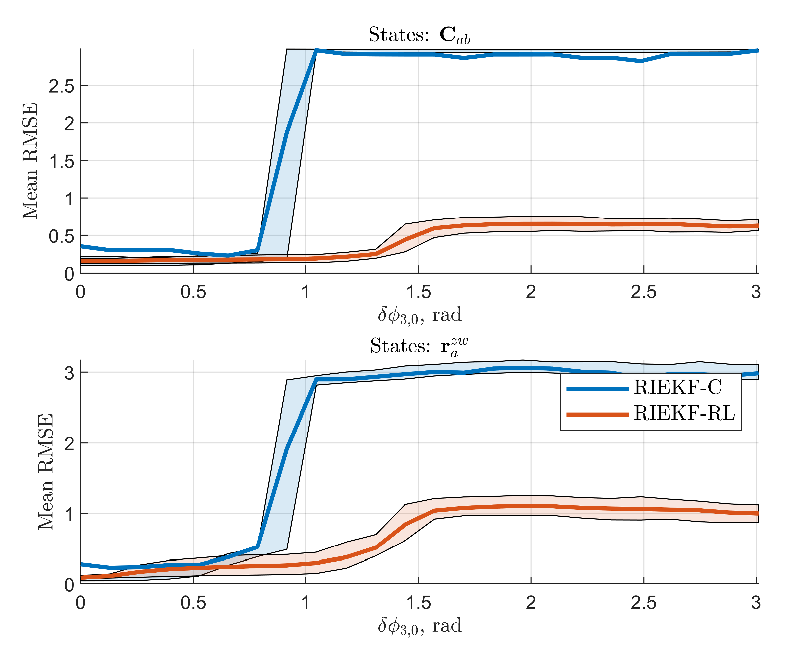
\includegraphics[width=\textwidth]{figs/se3/real/comp_att_rmse_state_Att_RL_C.eps}
		\caption{Mean RMSE for each state.}
	\end{subfigure}
	~
	\begin{subfigure}[b]{0.5\textwidth}
		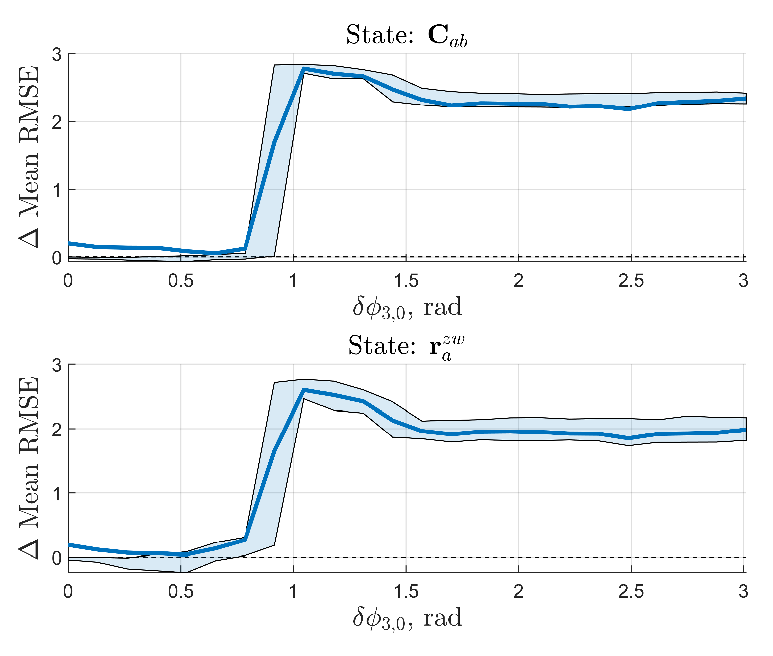
\includegraphics[width=\textwidth]{figs/se3/real/comp_att_diff_state_Att_RL_C.eps}
		\caption{Difference in mean RMSE of MEKF-R and RIEKF.}
	\end{subfigure}
	\caption[Results comparing the RIEKF-C and RIEKF-RL at different initial attitude errors.]{Results of 50 Monte Carlo trials comparing the RIEKF-C and RIEKF-RL at different initial attitude errors.}
	\label{fig:se3_comp_real_att_sim}
\end{figure} 

Based on these results, the error in the initial conditions were drawn from a zero-mean normal distribution with covariance $\mbf{P}_0 = \mathrm{diag}\left(0.1^2 \mbf{1}, \left(\f{\pi}{12}\right)^2\mbf{1}\right)$. The four filters are initially tested in simulation. The results of 500 MC simulations are shown in Figure~\ref{fig:se3_comp_real_sim}, where the error bars capture 80\% of the data. On average, the filters using the pseudo-measurements outperformed the sensors using the camera measurements directly. The RIEKF-C yielded a better attitude estimate than the MEKF-C, but a poorer position estimate.  This trend is repeated in the filters using the pseudo-measurements. However, there is significant spread in the results, as shown by the overlapping error bars. The RIEKF-C did indeed have a lower mean attitude RMSE than the MEKF-C, but it only outperformed the MEKF-C in 51.2\% of the trials. A similar trend is observed in the filters which use pseudo-measurments, where the RIEKF-RL outperformed the MEKF-RL in 53.2\% of the trials. The RIEKF does provide a better attitude estimate than the MEKF on average, but the impact is marginal. Running similar trials on real data reinforced some ideas from simulation. In particular, the MEKFs outperformed the IEKFs in position estimation. Furthermore, there was again little difference in the atittude estimate. These results are shown in Figure~\ref{fig:se3_comp_real}. Despite having a clearly higher mean RMSE, the RIEKF-C outperformed the MEFK-C in 45.6\% of the trials. Similarly, the RIEKF-RL outperformed the MEKF-RL 43\% of the time, the camera-based filters outperform the filters that use the pseudo-measurements.
\begin{figure}
	\centering
	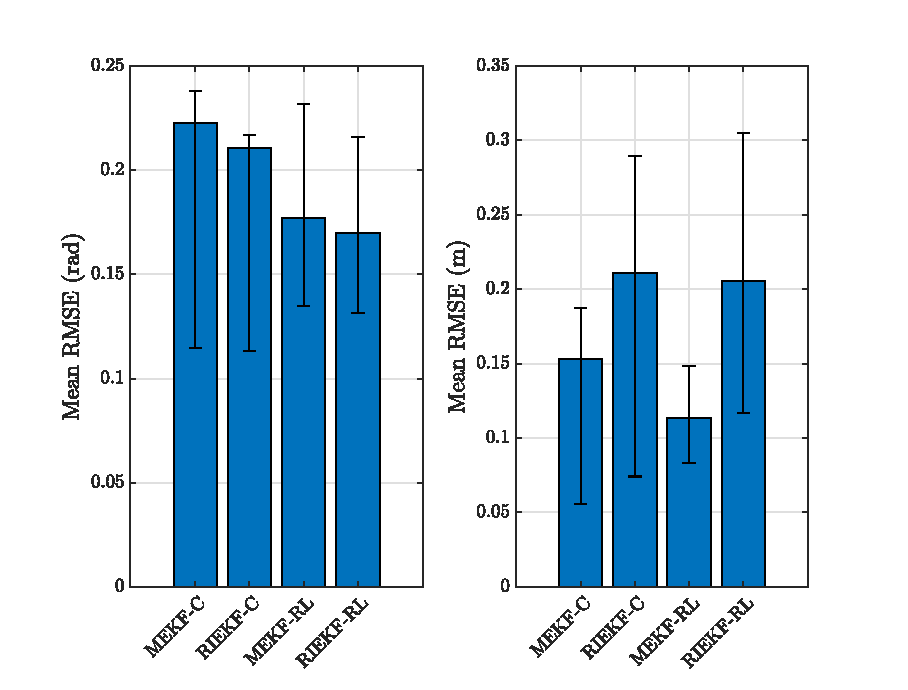
\includegraphics[width=0.7\textwidth]{figs/se3/real/comp_diff_state_sim.eps}
	\caption[Results comparing the MEKF-C, RIEKF-C, MEKF-RL, and RIEKF-RL on simulated data.]{Results of 500 Monte Carlo trials comparing the MEKF-C, RIEKF-C, MEKF-RL, and RIEKF-RL on simulated data. The mean RMSEs in attitude (left) and position (right) are shown.}
	\label{fig:se3_comp_real_sim}
\end{figure}
\begin{figure}
	\centering
	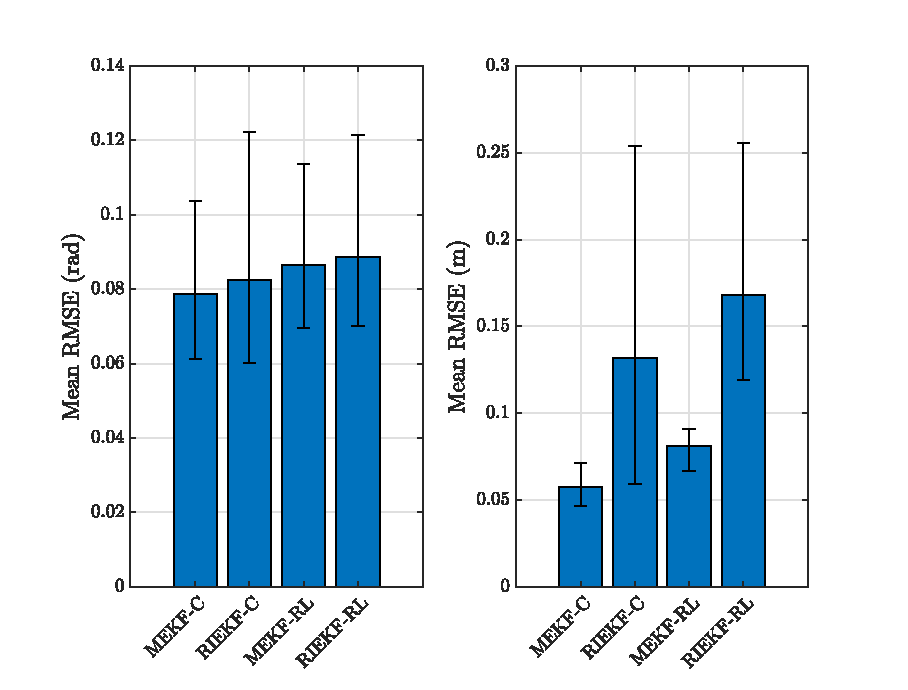
\includegraphics[width=0.7\textwidth]{figs/se3/real/comp_diff_state_Real.eps}
	\caption[Results comparing the MEKF-C, RIEKF-C, MEKF-RL, and RIEKF-RL on real data.]{Results of 500 Monte Carlo trials comparing the MEKF-C, RIEKF-C, MEKF-RL, and RIEKF-RL on real data. The mean RMSEs in attitude (left) and position (right) are shown.}
	\label{fig:se3_comp_real}
\end{figure}

\FloatBarrier

\section{Estimating Bias In the Invariant Framework}

In many estimation problems, sensor biases must be estimated. The IEKF is not particularly well suited for bias estimation, as including bias in the process model destroys the group-affine property. Despite this,  there still may be advantages to estimating bias in the invariant framework. To illustrate this, the sample problem is modified to include a time-varying bias in the rate gyro. For the sake of brevity, only the right-invariant model is shown. The rate gyro measurement model is now
\bdis
	\mbf{u}_b^1 = \mbs{\omega}_b^{ba} - \mbs{\beta}_b - \mbf{w}_b^1,
\edis
where the bias is modelled as a random walk with $\mbsdot{\beta}_b \sim \mc{N}(\mbf{0},\mbf{Q}^3)$.

The state can now be formulated as an element of a new matrix Lie group \cite{Heo2018}, $\mathcal{G}_1$. An element of $\mathcal{G}_1$ is
\bdis
	\mbf{X} = 
	\bma{cccc}
		\mbf{C}_{ab} & \mbf{r}_a^{zw} & & \\
		& 1 & & \\
		& & \mbf{1} & \mbs{\beta}_b\\	
		& & & 1  \\
	\ema.
\edis
The inverse is 
\bdis
	\mbf{X}^{-1} = 
	\bma{cccc}
		\mbf{C}_{ab} & -\mbf{C}_{ab}\mbf{r}_a^{zw} & & \\
		& 1 & & \\
		& & \mbf{1} & -\mbs{\beta}_b\\	
		& & & 1  \\
	\ema.
\edis
Let $\mathfrak{g}_1$ be the matrix Lie algebra of $\mc{G}_1$. The column matrix $\mbs{\xi} \in \mathbb{R}^{9}$ is mapped to $\mathfrak{g}_1$ using
\bdis
	\mbs{\xi}^\wedge = 
	\bma{c}
		\mbs{\xi}^\phi \\
		\mbs{\xi}^\textrm{r} \\
		\mbs{\xi}^\beta \\
	\ema^\wedge
	= 
	\bma{cccc}
		{\mbs{\xi}^\phi}^\times & \mbs{\xi}^\textrm{r} & & \\
		& 0 & & \\
		& & \mbf{0} & \mbs{\xi}^\beta \\	
		& & & 0  \\
	\ema.
\edis
The exponential map from $\mathfrak{g}_1$ to $\mc{G}_1$ is 
\bdis
	\expmapw{\mbs{\xi}} =
	\bma{cccc}
		\exp_{SO(3)}\left({\mbs{\xi}^\phi}^\times\right) & \mbf{J}\mbs{\xi}^\textrm{r} & & \\
		& 1 & & \\
		& & \mbf{1} & \mbs{\xi}^\beta \\	
		& & & 1  \\
	\ema,
\edis
where $\mbf{J}$ is given by \eqref{eq:SE3_Jac}. The adjoint representation of an element of $\mathcal{G}_1$ is
\bdis
	\textrm{Ad}(\mbf{X}) = 
	\bma{ccc}
		\mbf{C}_{ab} & \mbf{0} & \mbf{0} \\
		{\mbf{r}_a^{zw}}^\times\mbf{C}_{ab} & \mbf{C}_{ab} & \mbf{0} \\
		\mbf{0} & \mbf{0} & \mbf{1}
	\ema
\edis 
The kinematics in matrix form are 
\bdis
	\mbfdot{X} = \mbf{X}\mbs{\varpi}^\wedge,
\edis
where 
\bdis
	\mbs{\varpi} =
	\bma{c}
		\mbs{\omega}_b^{ba} \\
		\mbf{v}_b^{zw/a}  \\
		\mbf{0}
	\ema.
\edis
Substituting for the measurement model, 
\bdis
	\mbfdot{X} = \mbf{X}(\mbf{u}_b + \mbf{w}_b)^\wedge, \label{eq:se3_bias_kin}
\edis
where 
\bdis
	\mbf{u}_b =
	\bma{c}
		\mbf{u}_b^1 \\
		\mbf{u}_b^2  \\
		\mbf{0}
	\ema
\edis
and 
\bdis
	\mbf{w}_b =
	\bma{c}
		\mbf{w}_b^1 \\
		\mbf{w}_b^2  \\
		\mbf{w}_b^3
	\ema.
\edis
The kinematics \eqref{eq:se3_bias_kin} are not group affine due to the bias. Therefore, the process model Jacobians will depend on the state estimate. However, using an invariant error definition, the Jacobians can still be derived in a way that causes the Jacobians to be state dependent in different ways. Whether this is advantageous is a question to be answered, at least partially, in this section, and may depend on the problem. It will be tested on the $SE(3)$ sample problem in the right-invariant case, using the measurement model \eqref{eq:se3_meas_right}.

The right-invariant error between some estimated state $\mbfbar{X}$ and the true state $\mbf{X}$ is 
\begin{align*}
	\mbfdel{X} &= \mbfbar{X}\mbf{X}^{-1} \\ 
	&= 
	\bma{cccc}
		\mbfbar{C}_{ab} & \mbfbar{r}_a^{zw} & & \\
		& 1 & & \\
		& & \mbf{1} & \mbsbar{\beta}_b^1\\	
		& & & 1  \\
	\ema
	\bma{cccc}
		\mbf{C}_{ab}^\trans & -\mbf{C}_{ab}\mbf{r}_a^{zw} & & \\
		& 1 & & \\
		& & \mbf{1} & -\mbs{\beta}_b^1\\	
		& & & 1  \\
	\ema \\
	&= 
	\bma{cccc}
		\mbfbar{C}_{ab}\mbf{C}_{ab}^\trans & \mbfbar{r}_a^{zw} - \mbfbar{C}_{ab}\mbf{C}_{ab}^\trans\mbf{r}_a^{zw} & & \\
		& 1 & & \\
		& & \mbf{1} & \mbsbar{\beta}_b^1 -\mbs{\beta}_b^1\\	
		& & & 1  \\
	\ema \\
	&=
	\bma{cccc}
		\mbfdel{C} & \mbfdel{r}  & & \\
		& 1 & & \\
		& & \mbf{1} & \mbsdel{\beta} \\	
		& & & 1  \\
	\ema.
\end{align*}
Defining
\bdis
	\mbfhat{u}_b = 
	\bma{c}	
		\mbf{u}_b^1 + \mbshat{\beta}_b \\
		\mbf{u}_b^2 \\
		\mbf{0}
	\ema,
\edis
the right-invariant error propagation is
\begin{align*}
	\delta \mbfdot{X} &= \dot{\mbfhat{X}}\mbf{X}^{-1} + \mbfhat{X}\mbfdot{X}^{-1} \\ 
	&= \mbfhat{X}\mbfhat{u}_b^\wedge\mbf{X}^{-1} + \mbfhat{X}\mbf{X}^{-1}\mbfdot{X}\mbf{X}^{-1} \\
	&= \mbfhat{X}\mbfhat{u}_b^\wedge\mbf{X}^{-1} + \mbfhat{X}\mbf{X}^{-1}\mbf{X}(\mbf{u}_b + \mbf{w}_b)^\wedge\mbf{X}^{-1} \\
	&= \mbfhat{X}(\mbfhat{u}_b - \mbf{u}_b - \mbf{w}_b)^\wedge\mbf{X}^{-1} \\
	&= \mbfhat{X}(\mbfhat{u}_b - \mbf{u}_b - \mbf{w}_b)^\wedge\mbfhat{X}^{-1}\mbfhat{X}\mbf{X}^{-1} \\
	&= \left(\textrm{Ad}(\mbfhat{X})(\mbfhat{u}_b - \mbf{u}_b - \mbf{w}_b)\right)^\wedge\mbfdel{X}.
\end{align*}
To simplify, let
\begin{align*}
	\mbfdel{u} &= \mbfhat{u}_b - \mbf{u}_b \\
	&= 
	\bma{c}
		\mbf{u}_b^1 + \mbshat{\beta}_b \\
		\mbf{u}_b^2 \\
		\mbf{0}
	\ema -
	\bma{c}
		\mbf{u}_b^1 + \mbs{\beta}_b \\
		\mbf{u}_b^2 \\
		\mbf{0}
	\ema \\
	&=
	\bma{c}
		\mbsdel{\beta} \\
		\mbf{0} \\
		\mbf{0}
	\ema \\
	&= \mbf{B}\mbsdel{\xi},
\end{align*}
where 
\bdis
	\mbf{B} = 
	\bma{ccc}
		\mbf{0} & \mbf{0} & \mbf{1} \\
		\mbf{0} & \mbf{0} & \mbf{0} \\
		\mbf{0} & \mbf{0} & \mbf{0}
	\ema.
\edis
Linearizing by letting $\mbfdel{X} = \mbf{1} + \mbsdel{\xi}^\wedge$ and neglecting second order terms,
\begin{align*}
	\f{\dee}{\dt} \left(\mbf{1} + \mbsdel{\xi}^\wedge\right) &= \left(\textrm{Ad}(\mbfhat{X})(\mbf{B}\mbsdel{\xi} - \mbf{w}_b)\right)^\wedge(\mbf{1} + \mbsdel{\xi}^\wedge), \\
	\delta \mbsdot{\xi}^\wedge &= \left(\textrm{Ad}(\mbfhat{X})(\mbf{B}\mbsdel{\xi} - \mbf{w}_b)\right)^\wedge, \\
	\delta \mbsdot{\xi} &= \textrm{Ad}(\mbfhat{X})\mbf{B}\mbsdel{\xi} - \textrm{Ad}(\mbfhat{X})\mbf{w}_b.
\end{align*}
Therefore, $\mbf{A} = \textrm{Ad}(\mbfhat{X})\mbf{B}$ and $\mbf{L} = -\textrm{Ad}(\mbfhat{X})$. Explicitly,
\bdis
	\mbf{A} = 
	\bma{ccc}
		\mbf{0} & \mbf{0} & \mbfhat{C}_{ab} \\
		\mbf{0} & \mbf{0} & {\mbfhat{r}_a^{zw}}^\times\mbfhat{C}_{ab} \\
		\mbf{0} & \mbf{0} & \mbf{0}
	\ema.
\edis
The matrix $\mbf{A}$ depends on the state estimate because the process model is not group affine.

The innovation associated with the $i^{th}$ landmark is
\begin{align}
	\bma{c} \mbf{z}_k^i \\ \mbf{0} \ema &= \mbfcheck{X}_k\left(\bma{c} \mbf{y}_{b_k}^i \\ 1 \\ \mbf{0} \ema - \bma{c} \mbfcheck{y}_{b_k}^i \\ 1 \\ \mbf{0} \ema\right) \nonumber \\
	&= \mbfcheck{X}_k \left(\mbf{X}_k^{-1} \bma{c} \mbf{r}_a^{p_iw} \\	1 \\ \mbf{0} \ema + \bma{c} \mbf{v}_{b_k} \\ \mbf{0} \ema - \mbfch{X}_k^{-1} \bma{c} \mbf{r}_a^{p_iw} \\ 1  \\ \mbf{0}	\ema \right) \nonumber \\
	&= \delta \mbfch{T}_k \bma{c} \mbf{r}_a^{p_iw} \\	1 \ema + \mbfch{T}_k\bma{c} \mbf{v}_{b_k} \\0 \ema - \bma{c} \mbf{r}_a^{p_iw} \\ 1 \ema. \label{eq:se3_right_bias_3}
\end{align}
Linearizing \eqref{eq:se3_right_bias_3} by letting  $\delta \mbfcheck{X}_k \approx \mbf{1} + \delta \mbscheck{\xi}_k^\wedge$ and $\mbf{v}_{b_k} = \mbfdel{v}_{b_k}$,
\begin{align}
	\bma{c} \mbf{z}_k^i \\ \mbf{0} \ema &\approx \left(\mbf{1} + \delta \mbscheck{\xi}_k^\wedge\right) 
\bma{c}
	\mbf{r}_a^{p_iw} \\
	1 \\
	\mbf{0}
\ema +
\mbfcheck{X}_k
\bma{c}
	\mbfdel{v}_{b_k}^i \\
	\mbf{0}
\ema - 	
\bma{c}
	\mbf{r}_a^{p_iw} \\
	1 \\
	\mbf{0}
\ema \nonumber \\
	& = \delta \mbscheck{\xi}_k^\wedge 
\bma{c}
	\mbf{r}_a^{p_iw} \\
	1 \\
	\mbf{0}
\ema + \mbfcheck{X}_k
\bma{c}
	\mbfdel{v}_{b_k}^i \\
	\mbf{0}
\ema \nonumber \\
	& =  
\bma{cc}
	{\delta\mbscheck{\xi}^{\phi}}^\times & \delta\mbscheck{\xi}_k^\textrm{r} \\
 	\mbf{0} & 0 
\ema 
\bma{c}
	\mbf{r}_a^{p_iw} \\
	1 \\
	\mbf{0}
\ema + \mbfcheck{X}_k
\bma{c}
	\mbfdel{v}_{b_k}^i \\
	\mbf{0}
\ema \nonumber \\
	& =  
\bma{c}
	{\delta\mbscheck{\xi}^{\phi}}^\times\mbf{r}_a^{p_iw} + \delta\mbscheck{\xi}_k^\textrm{r} \\
 	\mbf{0} 
\ema 
 + \mbfcheck{X}_k
\bma{c}
	\mbfdel{v}_{b_k}^i \\
	\mbf{0}
\ema \nonumber \\
	& =  
\bma{c}
	-{\mbf{r}_a^{p_iw}}^\times{\delta\mbscheck{\xi}^{\phi}} + \delta\mbscheck{\xi}_k^\textrm{r} \\
 	\mbf{0} 
\ema 
 + \mbfcheck{X}_k
\bma{c}
	\mbfdel{v}_{b_k}^i \\
	\mbf{0}
\ema \nonumber \\
	& =  
	\mbftilde{H}^i \delta \mbscheck{\xi}_k + \mbfcheck{X}_k
\bma{c}
	\mbfdel{v}_{b_k}^i \\
	\mbf{0}
\ema , \label{eq:se3_right_bias_4}
\end{align}
where 
\bdis
	\mbftilde{H}^i = 
	\bma{ccc}
		-{\mbf{r}_a^{p_iw}}^\times & \mbf{1} & \mbf{0} \\
		\mbf{0} & \mbf{0} & \mbf{0}
	\ema.
\edis
Noting that the bottom row of \eqref{eq:se3_right_bias_4} is always $\mbf{0}$, it can be written
\bdis
	\mbf{z}_k^i = \mbf{H}^i \delta \mbscheck{\xi}_k + \mbf{M}_k^i \mbfdel{v}_{b_k}^i
\edis
where
\bdis
	\mbf{H}^i = 
	\bma{ccc}
		-{\mbf{r}_a^{p_iw}}^\times & \mbf{1} & \mbf{0} \\
	\ema
\edis
and $\mbf{M}_k^i = \mbfch{C}_{ab_k}^\trans$. For the $m$ landmarks,
\beq
	\mbf{H} = \underset{i = 1,\ldots,m}{\textrm{row}}\left(
	\bma{cc}
		-{\mbf{r}_a^{p_iw}}^\times & \mbf{1} \\
	\ema
	\right) \label{eq:se3_H_riekf_bias}
\eeq
and $\mbf{M}_k = \textrm{diag}\left(\mbfcheck{C}_{ab_k}^\trans,\ldots,\mbfcheck{C}_{ab_k}^\trans\right)$. In this case, $\mbf{H}$ is state independent.

\subsection{MEKF Solution}

Similar to Section~\ref{ssec:se3_EKF}, the RIEKF is compared to an MEKF. The MEKF errors are defined as $\mbfdel{C} = \mbfbar{C}_{ab}^\trans\mbf{C}_{ab}$, $\mbfdel{r} = \mbf{r}_a^{zw} - \mbfbar{r}_a^{zw}$, and $\mbsdel{\beta}_b = \mbs{\beta}_b - \mbsbar{\beta}_b$. The MEKF process model Jacobians are
\bdis
	\mbf{A} =
	\bma{ccc} 
		-{\mbf{u}_b^1}^\times & \mbf{0} & \mbf{1} \\
		-\mbfhat{C}_{ab}{\mbf{u}_b^2}^\times & \mbf{0} & \mbf{0} \\
		\mbf{0} & \mbf{0} & \mbf{0}
	\ema
\edis
and $\mbf{L} = \mbf{1}$, while the measurement Jacobians are
\bdis
	\mbf{H}_k = \underset{i = 1,\ldots,m}{\textrm{row}}\left(
	\bma{ccc}
		  \left(\mbfch{C}_{ab_k}^\trans\left( \mbf{r}_a^{p_iw} - \mbfch{r}_a^{z_k^iw} \right)\right)^\times & -\mbfch{C}_{ab_k}^\trans & \mbf{0} \\
	\ema
	\right)
\edis
and $\mbf{M}_k = \mbf{1}$.

\subsection{Simulation Results}

The MEKF and RIEKF are compared in simulation. The noise standard deviations are the same as those in Table~\ref{tab:se3_noises}. In addition, the noise in the bias random walk is assumed isotropic, $\mbf{Q}_k^3 = {\sigma_k^3}^2\mbf{1}$ and is set to $\sigma_k^3 = 0.005\mbf{1}$ \si{rad/s}. The error in the initial conditions were drawn from a zero-mean normal distribution with covariance $\mbf{P}_0 = \mathrm{diag}\left(0.1^2 \mbf{1}, \left(\f{\pi}{4}\right)^2\mbf{1},0.01^2\mbf{1}\right)$. The results obtained from varying the noise in the gyro, velocity sensors, landmark sensor and all the sensors simultaneously  are shown in Figures~\ref{fig:se3_comp_bias_gyro}~to~\ref{fig:se3_comp_bias_all}. On average, the RIEKF outperforms the MEKF, but the improvement is not as stark as when bias wasn't being estimated. This is due to the states now appearing in the process model Jacobian. However, as the measurement model Jacobians are independent of the state estimate, there is still an advantage to using the RIEKF.
\begin{figure}
	\centering
	\begin{subfigure}[b]{0.5\textwidth}
		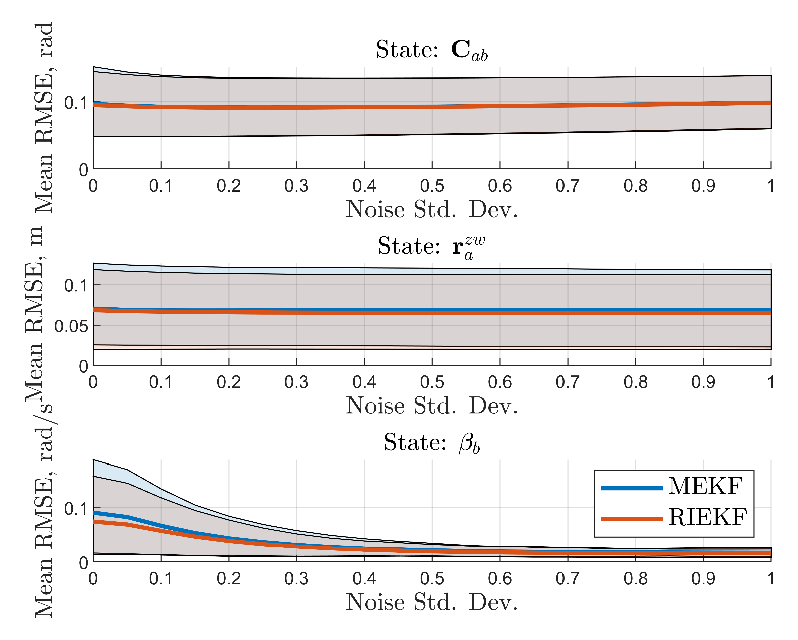
\includegraphics[width=\textwidth]{figs/se3/bias/comp_noise_rmse_state_Bias_Gyro_R.eps}
		\caption{Mean RMSE for each state.}
	\end{subfigure}
	~
	\begin{subfigure}[b]{0.5\textwidth}
		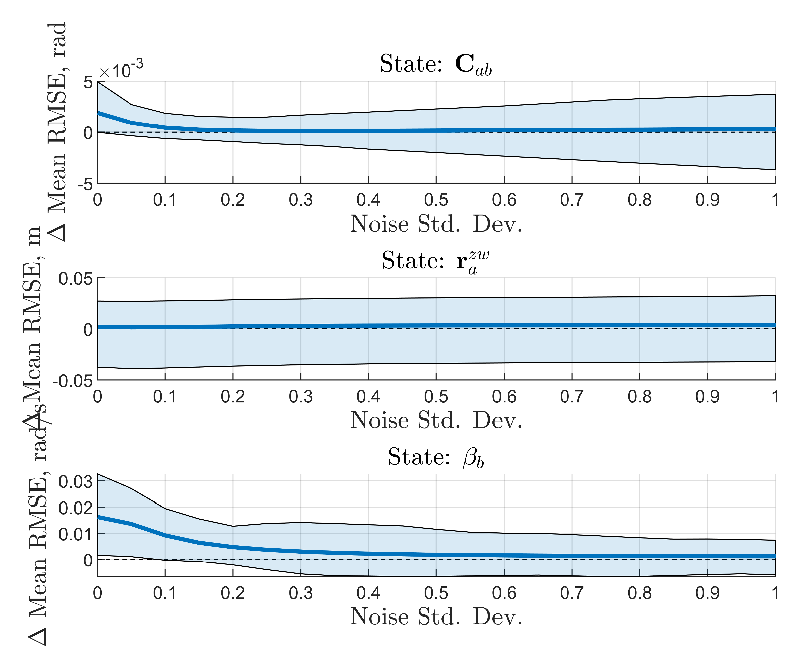
\includegraphics[width=\textwidth]{figs/se3/bias/comp_noise_diff_state_Bias_Gyro_R.eps}
		\caption{Difference in mean RMSE of MEKF and RIEKF.}
	\end{subfigure}
	\caption[Results comparing the MEKF-R and RIEKF varying rate gyro noise.]{Results of 50 Monte Carlo trials comparing the MEKF and RIEKF, where the noise in the rate gyro was varied.}
	\label{fig:se3_comp_bias_gyro}
\end{figure} 

\begin{figure}
	\centering
	\begin{subfigure}[b]{0.5\textwidth}
		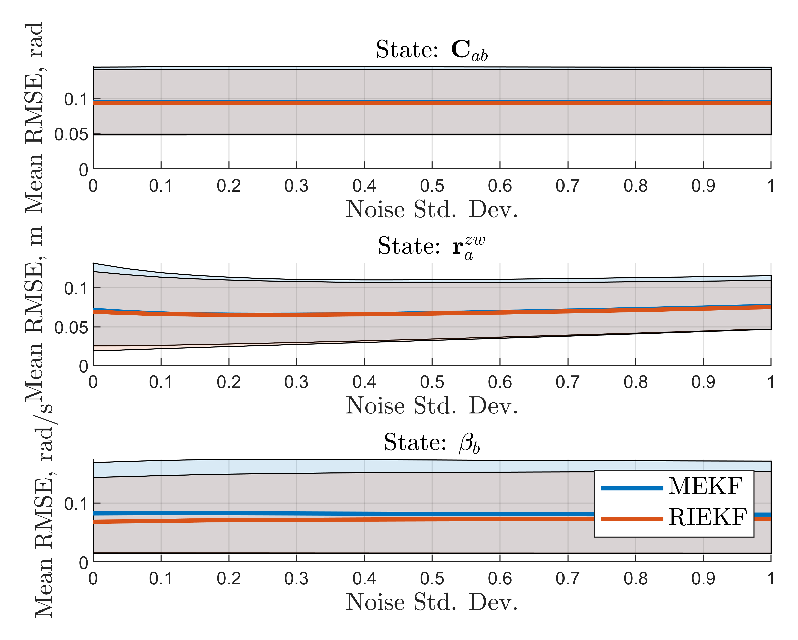
\includegraphics[width=\textwidth]{figs/se3/bias/comp_noise_rmse_state_Bias_Vel_R.eps}
		\caption{Mean RMSE for each state.}
	\end{subfigure}
	~
	\begin{subfigure}[b]{0.5\textwidth}
		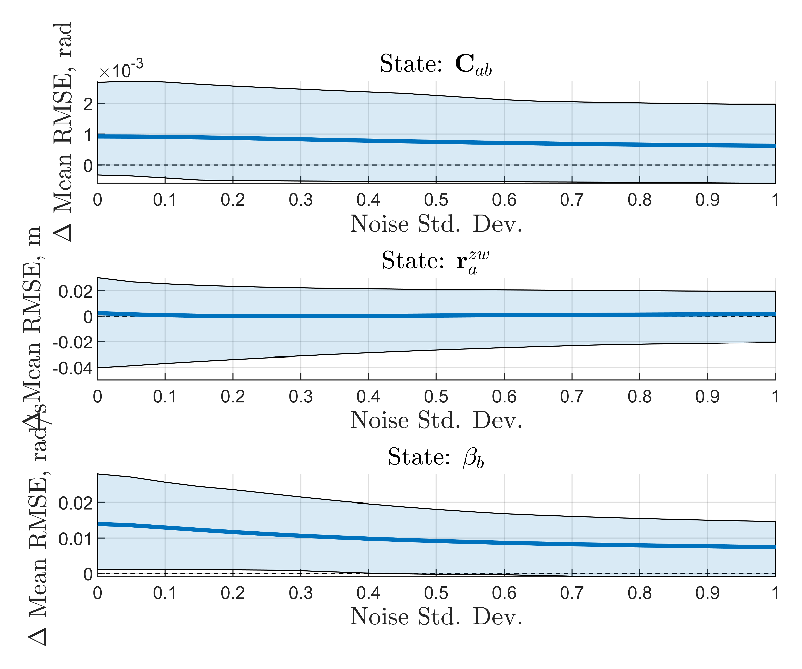
\includegraphics[width=\textwidth]{figs/se3/bias/comp_noise_diff_state_Bias_Vel_R.eps}
		\caption{Difference in mean RMSE of MEKF and RIEKF.}
	\end{subfigure}
	\caption[Results comparing the MEKF-R and RIEKF varying velocity sensor noise.]{Results of 50 Monte Carlo trials comparing the MEKF and RIEKF, where the noise in the velocity sensor was varied.}
	\label{fig:se3_comp_bias_vel}
\end{figure} 


\begin{figure}
	\centering
	\begin{subfigure}[b]{0.5\textwidth}
		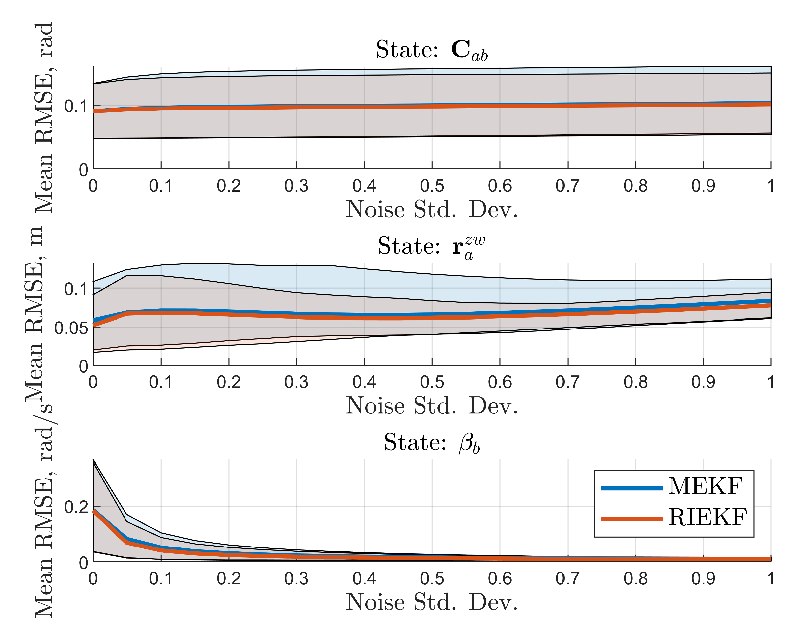
\includegraphics[width=\textwidth]{figs/se3/bias/comp_noise_rmse_state_Bias_Corr_R.eps}
		\caption{Mean RMSE for each state.}
	\end{subfigure}
	~
	\begin{subfigure}[b]{0.5\textwidth}
		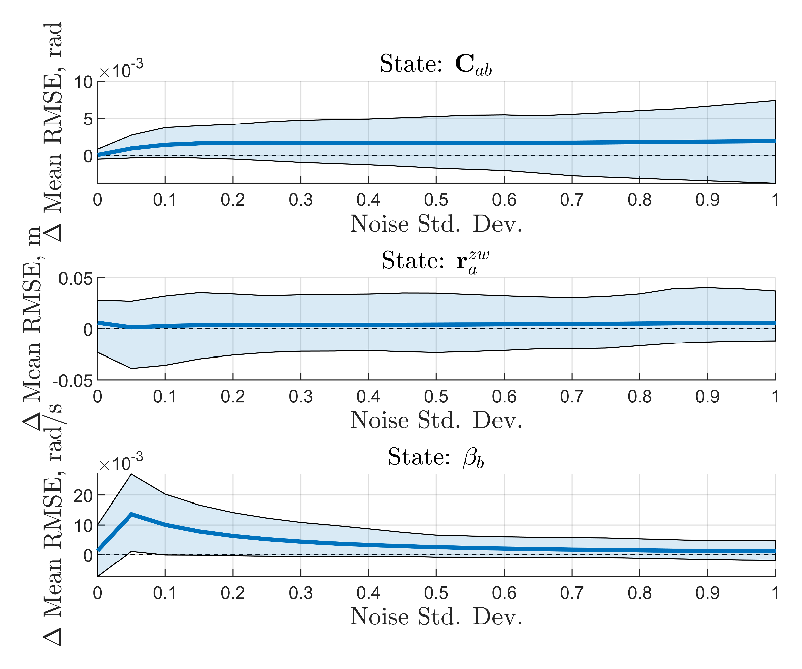
\includegraphics[width=\textwidth]{figs/se3/bias/comp_noise_diff_state_Bias_Corr_R.eps}
		\caption{Difference in mean RMSE of MEKF and RIEKF.}
	\end{subfigure}
	\caption[Results comparing the MEKF-R and RIEKF varying landmark sensor noise.]{Results of 50 Monte Carlo trials comparing the MEKF and RIEKF, where the noise in the landmark sensor was varied.}
	\label{fig:se3_comp_bias_corr}
\end{figure} 

\begin{figure}
	\centering
	\begin{subfigure}[b]{0.5\textwidth}
		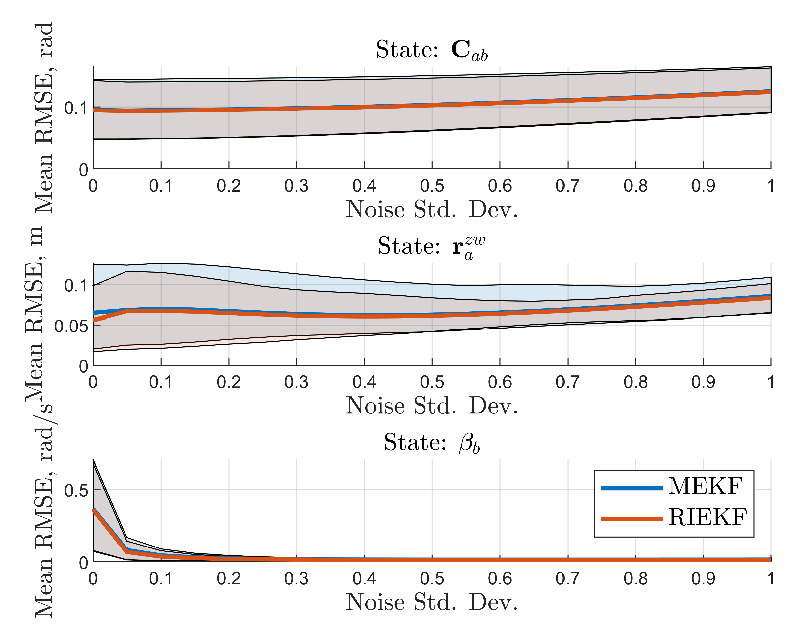
\includegraphics[width=\textwidth]{figs/se3/bias/comp_noise_rmse_state_Bias_All_R.eps}
		\caption{Mean RMSE for each state.}
	\end{subfigure}
	~
	\begin{subfigure}[b]{0.5\textwidth}
		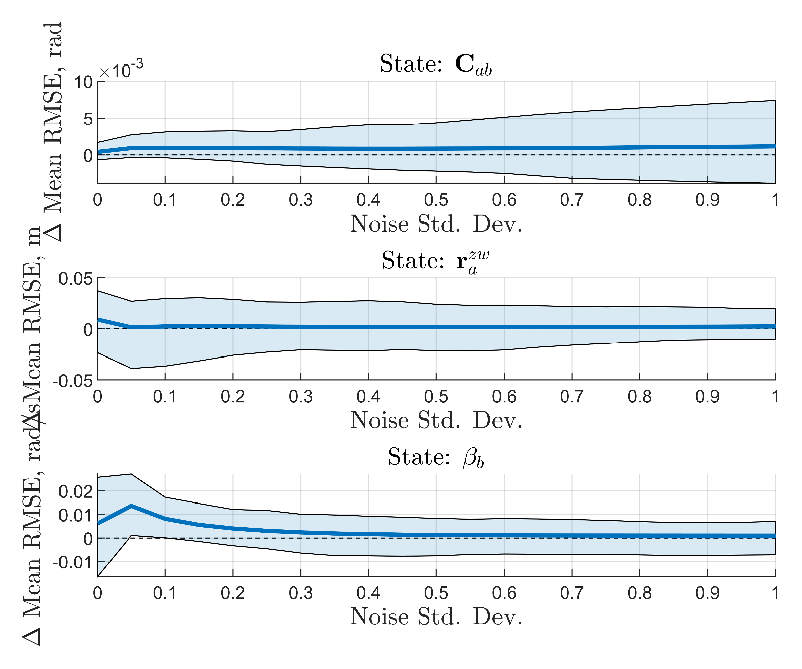
\includegraphics[width=\textwidth]{figs/se3/bias/comp_noise_diff_state_Bias_All_R.eps}
		\caption{Difference in mean RMSE of MEKF and RIEKF.}
	\end{subfigure}
	\caption[Results comparing the MEKF-R and RIEKF varying all sensor noise.]{Results of 50 Monte Carlo trials comparing the MEKF and RIEKF, where the noise in all the sensors varied.}
	\label{fig:se3_comp_bias_all}
\end{figure} 


\section{Conclusion}

In the introduction to this chapter, a set of questions were presented to guide an in-depth discussion on the practical implications of the IEKF. It is useful to revisit these questions at the end of this chapter. 

\begin{enumerate}
	\item \emph{Given a left-invariant measurement model, is it more advantageous to use a LIEKF than an MEKF, and given a right-invariant measurement model, is it more advantageous to use a RIEKF than an MEKF?}
	
	\item \emph{What is the effect of process and measurement noise? How quickly do the convergence properties of the IEKF claimed in \cite{Barrau2017,Barrau2018} break down?}
	
\end{enumerate}

The first two questions posed regarded the perfomance of the IEKF relative to a standard MEKF. In general, over all the experimental trials, the IEKF outperformed the MEKF. However, a more in-depth analysis revealed that much of the improvement could be attributed to better performance in the transient, as it is during this time that the Jacobians in the IEKF are much more accurate than those of the MEKF. During these trials, the effect of sensor noise was also isolated. Despite the convergence properties holding only when noise is negelected, the IEKF is still more effective than the MEKF in the presence of noise.

\begin{enumerate}
	\setcounter{enumi}{2}
	\item \emph{How can the IEKF be used in situations when the measurement model isn't left or right-invariant?}
	
\end{enumerate}

A realistic stereo camera measurement model was used to demonstrate how the IEKF can be used when the measurement model is neither left nor right-invariant. In this scenario, the RIEKF and MEKF provided similar performance, due to the fact that the measurement model was not exactly right-invariant. This was seen both when modifying the IEKF to use the raw measurements, and preprocessing the measurements to create right-invariant pseudomeasurements.

\begin{enumerate}
	\setcounter{enumi}{3}
	\item \emph{How can bias estimation be performed in an invariant framework?}
	
\end{enumerate}

 Lastly, bias estimation was performed in the invariant framework, using results from \cite{Barrau2015}, \cite{Hartley2018} and \cite{Heo2018}. The RIEKF provided better performance than the MEKF, but to a lesser degree than previously shown due to the process model no longer being group affine.